\chapter{Integrasjon i flere dimensjoner}
\label{chap:Integrasjon}
I dette kapittelet diskuteres integrasjon av funksjoner med flere variabler og vi skal integrere over områder i flerdimensjonale rom. Vi bygger direkte videre på Riemannsum-tankegangen fra énvariabeltilfellet (repetert i kapittel 0): vi ser for oss integralet som en grenseverdi av en sum av rektangelarealer.

\paragraph{Ved integrasjon i to dimensjoner} (eller flere for den saks skyld) får vi tilsvarende type summer, bare at vi nå summerer bidrag over et areal (eller volum) i stedet for et intervall. Men la oss aller først se på noen anvendelser av to-variable integraler.

\subsection*{Anvendelse: volum under en flate} 
Anta at vi ønsker å beregne volum under en flate gitt som graf til en funksjon
\[h \colon [-1,1] \times [-1,1] \rightarrow \R\quad,\quad h(x,y)=2-(x^2+y^2)\]
av to variabler. Vi lurer på hva volumet mellom grafen og $xy$-planet er. Grafen til funksjonen er vist i figur~\ref{fig:1}.
\begin{figure}[ht]
\begin{center}
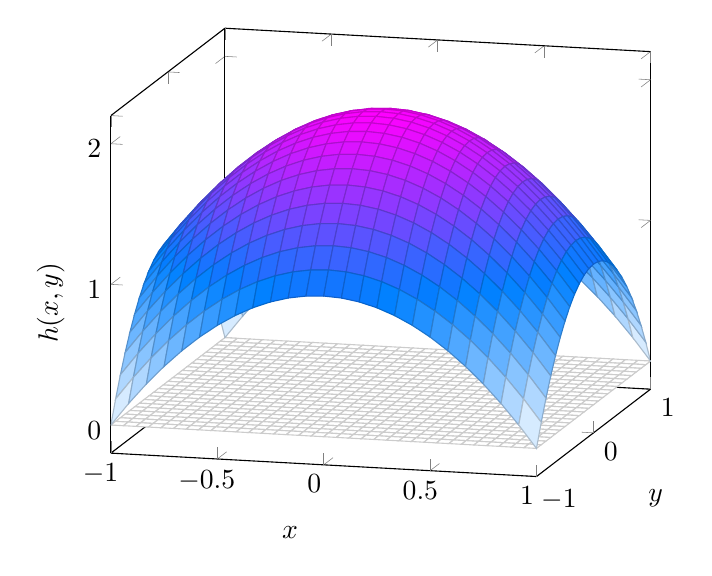
\begin{tikzpicture}
\begin{axis}[
    view={15}{15},
    domain=-1:1,
    y domain=-1:1,
    xlabel=$x$, ylabel=$y$, zlabel={$h(x,y)$},
    colormap/cool,
    mesh/ordering=y varies,
    samples=25,
    samples y=25,
]\addplot3[surf, domain=-1:1, samples=35] 
{0};
\addplot3[surf] 
{2-(x^2+y^2)};
\end{axis}
\end{tikzpicture}
\end{center}
  \caption{Graf til $h(x,y)=2-x^2-y^2$}
    \label{fig:1}
\end{figure}

Fra figur~\ref{fig:1} ser vi at området mellom grafen til $h(x,y)$ og $xy$-planet er et volum. Vi skriver
\[V=\iint_D h(x,y) dA,\]
hvor $D$ er integrasjonsdomenet i $xy$-planet slik som angitt i teksten over. Siden $xy$-planet består av to retninger bruker vi to integraltegn. Som vi skal se må vi nemlig integrere langs to retninger, eller variabler: Fra figuren ser vi at integrasjonsdomenet kan deles opp i små elementer $\Delta A$ som alle har sidekanter \(\Delta x\) og \(\Delta y\), altså at

\[\Delta A=\Delta x\cdot\Delta y.\]

Volumet av én enkelt søyle under grafen blir da

\[\Delta V_i= h(x_i^*,y_i^*)\cdot \Delta x\Delta y.\]

En approksimering til det totale volumet $V$ mellom grafen og $xy$-planet må derfor kunne uttrykkes som en dobbel Riemann-sum, analogt med 1D-tilfellet. Vi får

\[V\approx h(x_1^*,y_1^*) \Delta x \Delta y + h(x_2^*,y_2^*) \Delta x \Delta y + \cdots + h(x_n^*,y_n^*) \Delta x\Delta y = \sum_{i=1}^n\sum_{j=1}^m h(x_i^*,y_j^*)\Delta x\Delta y.\]
Om vi nå tar grenseverdien og lar $n,m\to \infty$ får vi integralet over. Vi skriver at

\[\iint_D h(x,y) dA=\int_{-1}^{1}\int_{-1}^1 h(x,y)dxdy = \lim_{n,m\to \infty}\sum_{i=1}^n\sum_{j=1}^m f(x_i^*,y_j^*)\Delta x\Delta y,\]
hvor vi her valgte å sette inn de spesifikke integrasjonsgrensene for dette eksemplet. Men resultatet gjelder selvsagt også tilsvarende for generelle integrasjonsgrenser. Dette kommer vi tilbake til i neste delkapittel. Merk at tankegangen også lett kan generaliseres til integraler i $n$ variabler.

\subsection*{Anvendelse: vanntrykk på demning}
En ingeniør som er involvert i byggingen av en demning for å holde tilbake vannet i et reservoar, må kunne beregne den totale kraften vannet utøver på demningen, slik at demningen bygges med tilstrekkelig styrke.
\Cref{fig:reservoar} viser situasjonen.

For å kunne beregne denne kraften må vi bruke følgende ingredienser:
\begin{enumerate}
  \item Vanntrykket \( p \) er proporsjonalt med dybden. Det vil si
  \begin{equation}
    p = kd \label{eq:pressure}
  \end{equation}
  der \( k \) er en konstant\footnote{Kanskje husker du fra fysikken at konstanten er $k=\rho\cdot\textrm{g}$, hvor $\rho$ er massetettheten til vannet og $\textrm{g}=9.81\,\textrm{m}/\textrm{s}^2$ er tyngdens akselerasjon.}.
  \item Kraften $\vect{F}$ på et areal $\vect{A}$ som utsettes for konstant trykk $p$, er gitt ved
  \begin{align}
&\text{kraft} =\text{trykk} \cdot \text{areal}\nonumber\\
&\vect{F}\quad=\quad p\quad\cdot\quad\vect{A},
\label{eq:kraftformel}
  \end{align}
  hvor $\vect{A}$ her er en vektor som står normalt på arealet, og med størrelse $A$.
\end{enumerate}
Dersom vi legger inn et koordinatsystem med origo ved bunnen av reservoaret, kan vi lett vise at vanndybden blir \( d=h-z \), og \( \Delta A \) er et lite areal på demningens overflate (se figur~\ref{fig:reservoar}).

\begin{figure}[ht]\centering
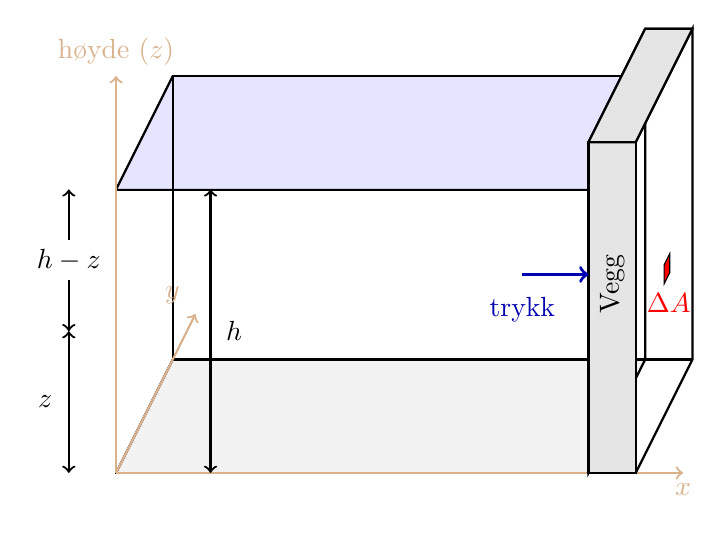
\begin{tikzpicture}[scale=1.2, x={(1cm,0cm)}, y={(0.3cm,0.6cm)}, z={(0cm,1cm)}]

% Dimensions
\def\H{3}    % Total height h
\def\L{5}    % Length in x-direction
\def\z{1.5}  % Arbitrary local height z

% Draw the front rectangle (wall)
\draw[thick] (0,0,0) -- (\L,0,0) -- (\L,0,\H) -- (0,0,\H) -- cycle;

%Shade bottom and top
\draw[fill=gray!10] (0,0,0) -- (\L,0,0) -- (\L,2,0) -- (0,2,0) -- cycle;
\draw[fill=blue!10] (0,0,\H) -- (\L,0,\H) -- (\L,2,\H) -- (0,2,\H) -- cycle;
% Vertical sides (walls)
\draw[thick] (\L,0,\H) -- (\L,2,\H) -- (\L,2,0) -- (\L,0,0) -- cycle;

\draw[thick] (0,0,\H) -- (0,2,\H);
\draw[thick] (0,0,0) -- (0,2,0);

% Back rectangle
\draw[thick] (0,2,0) -- (\L,2,0) -- (\L,2,\H) -- (0,2,\H) -- cycle;

% Axes
\draw[->, thick, brown!60!white] (0,0,0) -- (1.2*\L,0,0) node[anchor=north] {$x$};
\draw[->, thick, brown!60!white] (0,0,0) -- (0,2.8,0) node[anchor=south east, xshift=-2pt] {$y$};
\draw[->, thick, brown!60!white] (0,0,0) -- (0,0,1.4*\H) node[anchor=south] {høyde ($z$)};

%Reservoire wall
\draw[thick] (\L+.5,0,\H+.5) -- (\L+.5,2,\H+.5) -- (\L+.5,2,0) -- (\L+.5,0,0) -- (\L, 0,0) -- (\L, 0,\H+.5) -- (\L, 2,\H+.5) -- (\L+.5, 2,\H+.5);
\draw[thick,fill=gray!20] (\L,0,\H+.5) -- (\L+.5,0,\H+.5) -- (\L+.5,0,0) -- (\L,0,0) -- cycle;
\draw[thick,fill=gray!20] (\L,0,\H+.5) -- (\L+.5,0,\H+.5) -- (\L+.5,2,\H+0.5) -- (\L,2,\H+.5) -- cycle;
\draw[thick] (\L,2,0)--(\L+.5,2,0);
\node[rotate=90] at (\L+.25, 0,2) {Vegg};

% Height h and arrows
\draw[<->,thick] (1,0,0) -- (1,0,\H);
\node at (1.25,0,\H/2) {$h$};
\draw[<->,thick] (-.5,0,0) -- (-.5,0,\z);
\node at (-0.75,0,\z/2) {$z$};

\draw[<->,thick] (-.5,0,\z) -- (-.5,0,\H);
\node[fill=white] at (-0.5,0,{(\z+\H)/2}) {$h - z$};

% Area element (colored red)
\draw[fill=red] (\L+.5,1,\z-.1) -- (\L+.5,1,\z+.1) -- (\L+.5,1.2,\z+.1) -- (\L+.5,1.2,\z-.1) -- cycle;
\node[red] at ({\L + 0.7},.5,{\z}) {$\Delta A$};

% Pressure arrow on wall
\draw[->, thick, blue!70!black, line width=1.2pt] 
    ({\L-1}, 1, {\z}) -- ++(.7, 0, 0);
\node[blue!70!black] at  ({\L-1}, 1, {.75*\z}) {trykk};
\end{tikzpicture}
\caption{Skjematisk oversikt over reservoaret}\label{fig:reservoar}
\end{figure}
Ved å bruke \eqref{eq:pressure}, er trykket ved \( \Delta A \sim k(h - z) \). Ved å bruke \eqref{eq:kraftformel}, er (størrelsen på) kraften på et lite areal \( \Delta A\) nå gitt som \( \Delta F= k(h - z)\Delta A \). Begge disse uttrykkene er tilnærminger, siden \( y \) varierer litt fra toppen til bunnen av \( \Delta A \). Nå har vi:
\begin{align*}
\text{Total kraft} &= \text{summen av kreftene på alle } \Delta A \text{ som utgjør overflaten} \\
\rightarrow F &\approx \sum_{\text{alle } \Delta A} k(h - z)\Delta A
\end{align*}

For en bedre tilnærming lar vi \( \Delta A \) bli mindre, og for det eksakte resultatet finner vi grensen når \( \Delta A \to 0 \). Som i forrige eksempel finner vi også her et dobbeltintegral, denne gangen for størrelsen til kraften:

\[F=\iint_Dk(h-z)dzdy.\]
Her er $D$ ment å være demningens utstrekning i $zy$-planet.

\paragraph{I begge eksemplene} over på anvendelser var det nødvendig å summere en størrelse over et areal. Summene som opptrer ser ut som Riemannsummer. 


For funksjoner av én variabel integrerte vi over et intervall (et én-dimensjonalt rom). Da gir det mening at vi for funksjoner av \textit{to variabler} integrerer over et område i planet, altså et \textit{to-dimensjonalt rom}.


\subsection*{Formelt: Integrasjon over et rektangulært domene}
Vi begynner med å anta at det todimensjonale området \( R \) er et rektangel, definert som:
\[
R = [a, b] \times [c, d].
\]
Det betyr at \( x \) varierer fra \( a \) til \( b \), og \( y \) fra \( c \) til \( d \).
La oss nå se på grafen til flaten \( z = f(x, y) \) over rektangelet \( R \). Akkurat som for én variabel: hva er volumet\footnote{Strengt tatt må vi anta at $f(x,y)>0$ for denne tolkningen, eller i alle fall kreve at $f(x,y)$ ikke bytter fortegn over $R$.} under \( f(x, y) \) og over \( xy \)-planet?

Vi tilnærmer volumet på samme måte som vi tilnærmet arealet før. Del opp \( [a, b] \) i \( n \) delintervaller og \( [c, d] \) i \( m \) delintervaller. Dette deler opp \( R \) i mindre rektangler. Fra hvert rektangel velger vi et punkt \( (x_i^*, y_j^*) \). Over hvert av disse rektanglene konstruerer vi en boks med høyde \( f(x_i^*, y_j^*) \). Grunnflatens areal er \( \Delta A \), og volumet av hver boks er:
\(
f(x_i^*, y_j^*) \Delta A
\)
Volumet under flaten er tilnærmet:
\[
V \approx \sum_{i=1}^n \sum_{j=1}^m f(x_i^*, y_j^*) \Delta A
\]
For å få eksakt volum, lar vi \( n, m \to \infty \):

\[
V = \lim_{n, m \to \infty} \sum_{i=1}^n \sum_{j=1}^m f(x_i^*, y_j^*) \Delta A
\]

Dette er definisjonen på et dobbeltintegral av en funksjon av to variable:

\begin{defn}{Dobbeltintegral over et rektangel}
La \( R \) være et rektangel og $f$ en funksjon definert på \(R\). Da definerer vi
\[
\iint_R f(x, y) \, dA = \lim_{n, m \to \infty} \sum_{i=1}^n \sum_{j=1}^m f(x_i^*, y_j^*) \Delta A
\]
Hvor \( dA = dx\, dy \) kalles \emph{differensialarealet}. Merk at i denne notasjonen har vi ingen grenser på integraltegnene, men området \( R \) er angitt under integral-tegnene.
\end{defn}

\begin{rem}{Tolkning av dobbeltintegral som volum}
En tolkning av dobbeltintegralet er volumet under funksjonen \( f(x, y) \geq 0\) og over \( xy \)-planet:
\[
\text{Volum} = \iint_R f(x, y) \, dA
\]
\textbf{OBS}:
Integralet gir et volum i fysisk forstand hvis $f(x,y)$, $dx$ og $dy$ har lengde som måleenheter og
$f(x,y)\geq 0$.  Det tilsvarer det bestemte integralet for en funksjon av en variabel $\int_a^b f(x)d x$ som gir et areal når $dx$ og $f(x)$ er lengder og $f(x)>0$. Hvis funksjonen ikke er positiv, må vi dele opp integrasjonsområdet og summere absoluttverdiene til integralene av delene.
\end{rem}
Definisjonen av dobbeltintegral ved hjelp av grenseverdier kan ikke brukes i praksis når vi må regne for hånd (men vi skal møte ideen igjen når vi lager numeriske metoder for integraler i \Cref{sect:num_met1}). I neste avsnitt skal vi lære hvordan vi kan forenkle beregning ved hjelp av de kjente endimensjonale integraler.

\section{Dobbeltintegraler i kartesiske koordinater}\label{sect:dobbelint}

I forrige delkapittel ga vi definisjonen på dobbeltintegralet ved hjelp av grenseverdier. I dette delkapitlet antar vi fremdeles at vi integrerer over et rektangel:
\[
R = [a, b] \times [c, d]
\]
Generelle områder behandler vi senere.
Neste resultat viser hvordan vi regner ut dobbeltintegraler over rektangulære områder i praksis.

\begin{thrm}{Fubinis teorem}
Dersom \( f(x, y) \) er kontinuerlig på \( R \) gjelder at
\[
\iint_R f(x, y) \, dA = \int_a^b \bigl(\int_c^d f(x, y) \, dy \bigr) \, dx = \int_c^d \bigl(\int_a^b f(x, y) \, dx \bigr) \, dy
\]
Disse integralene kalles \textbf{itererte integraler}. \label{thm:fubini}
\end{thrm}

\textbf{Merk:} 
\begin{itemize}
\item Det er vanlig å skrive de itererte integralene uten parenteser, som
$$\int_a^b \int_c^d f(x, y) \, dy  \, dx$$
hvor da $a$ og $b$ er grensene for integralet med
hensyn på $x$ og $c$ og $d$ er grensene for integralet
med hensyn på $y$.
\item 
Hvilket av de to itererte integralene (dvs. hvilken
rekkefølge vi velger) har ingenting å si for
verdien av integralet. Men det kan godt være at 
én rekkefølge gir enklere regning enn den andre. 
\end{itemize}

\begin{oppsum}{Hvordan beregner man dobbeltintegraler i praksis?}
For å regne ut dobbeltintegraler starter vi med det indre integralet. Vi holder den andre variabelen konstant og integrerer som om det var et vanlig én-variabelintegral.

Dette minner om partiellderivasjon, hvor vi behandler en variabel som konstant for å derivere med hensyn på den andre.
\end{oppsum}

\begin{eks}{Regn ut!}
Beregn følgende dobbeltintegraler over de gitte rektangler:
\begin{align*}
\text{(a) }&\iint_R xy^2 \, dA, \quad R = [0, 1] \times [1, 2]\\
\text{(b) }&\iint_R (x - y^3) \, dA, \quad R = [-1, 1] \times [0, 2]\\
\text{(c) }&\iint_R x e^{x^2 +y} \, dA, \quad R = [-1, 0] \times [0, 1]
\end{align*}
\textbf{OBS:} Alle funksjoner som integreres her er kontinuerlige. Dermed kan vi beregne ved hjelp av itererte integraler.
\end{eks}

\begin{oppsum}{Én-variable funksjoner i dobbeltintegral}
I noen tilfeller er funksjonen som integreres et produkt av funksjoner av én variabel. La oss se på funksjonen \( f(x, y) = g(x) h(y) \) hvor domenet er gitt ved \( R = [a, b] \times [c, d] \). Da har vi at
\[
\iint_R f(x, y) \, dA = \left( \int_a^b g(x) \, dx \right) \left( \int_c^d h(y) \, dy \right).
\]
Dette gjelder fordi man kan trekke ut ut én av funksjonene fra det indre integralet (husk: hvis noe er konstant kan vi trekke det ut av et integral!), og deretter utføre integrasjonen separat.
\end{oppsum}


\begin{eks}{Regn ut!}
Beregn:
\[
\iint_R  x e^{x^2 +y} \, dA, \quad R = [-1, 0] \times \left[0, 1\right]
\]
Siden $e^{x^2+y}=e^{x^2}e^y$ kan vi skrive integranden som et produkt, så:
\[
\left( \int_{-1}^{0} xe^{x^2} \, dx \right) \left( \int_0^{1} e^y \, dy \right) = \left.\frac{e^{x^2}}{2}\right|_{-1}^0 \left.e^y\right|_0^{1} = \frac{1}{2}(1-e)(e-1)=-\frac{1}{2}(e-1)^2 \simeq -1.4762
\]
\end{eks}

Så langt har vi bare diskutert bestemte integraler. I praksis kan det forekomme at vi ønsker å beregne ubestemte integraler og det forklarer vi nå:
\begin{eks}{Ubestemte integraler av to-variable funksjoner}
Anta at vi er nødt til å beregne integralene
\[
\int (2x \cos^2(y) + xy) \, dy, \quad \int (x - ye^{x}) \, dx
\]
med hensyn til én variabel. Her behandles den andre variabelen som en konstant. \textbf{OBS:} Integrasjonskonstanten må derfor være en funksjon av den andre variabelen.
\begin{align*}
\int (2x\cos^2 (y) + xy) \, dy = xy+x\sin(y)\cos(y) + \frac{1}{2}x y^2 + g(x)
\end{align*} 
På samme vis får vi
\begin{align*}
\int (x - ye^{x}) \, dx = \tfrac{1}{2} x^2 - y e^{x} + h(y).
\end{align*}
\end{eks}
\subsection{Dobbeltintegraler over generelle områder}

I forrige seksjon så vi på dobbeltintegraler over rektangler. Problemet med dette er at de fleste områder ikke er rektangulære. Vi ønsker derfor å studere integraler av formen:
\[
\iint_D f(x, y)\, dA
\]
hvor \( D \) kan ha en annen form enn et rektangel. Det vi skal se på er de såkalte standardområdene for integrasjon, hvor en begrensning av området er gitt ved hjelp av funksjoner som beskriver en side i $x$- eller $y$-retning.

\begin{oppsum}{Standard integrasjonsområder}
Vi har to typer områder hvor den ene begrensningen i $x$- (eller $y$-)retning er avhengig av $y$- (eller $x$-)variabelen. For begge typene er definisjonen av integralet gitt som vist under:\footnote{I andre kilder brukes også betegnelsene \emph{Type 1} og \emph{Type 2} (eller \emph{Type I}/\emph{Type II}) om disse to områdetypene, se for eksempel \cite{Adams}. Vi bruker gjennomgående $y$-enkelt og $x$-enkelt i dette kompendiet.}
\begin{align*}
  \text{\textbf{$y$-enkelt: }} & & D = \{ (x, y) \mid a \leq x \leq b, \ g_1(x) \leq y \leq g_2(x) \} \\
  &&\iint_D f(x, y)\, dA := \int_a^b \int_{g_1(x)}^{g_2(x)} f(x, y)\, dy\, dx\\
  \text{\textbf{$x$-enkelt: }} & & D = \{ (x, y) \mid c \leq y \leq d, \ h_1(y) \leq x \leq h_2(y) \} \\
  && \iint_D f(x, y)\, dA := \int_c^d \int_{h_1(y)}^{h_2(y)} f(x, y)\, dx\, dy
\end{align*}
Se \Cref{fig:arealtyper} for en grafisk fremstilling. 

\begin{rem}{}
Den variable grensen kommer alltid i det indre integralet. 
\end{rem}
\end{oppsum}
\begin{figure}[ht]
\centering
\begin{tikzpicture}
  \node[inner sep=0, anchor=south west] (areatypesimg) at (0,0) {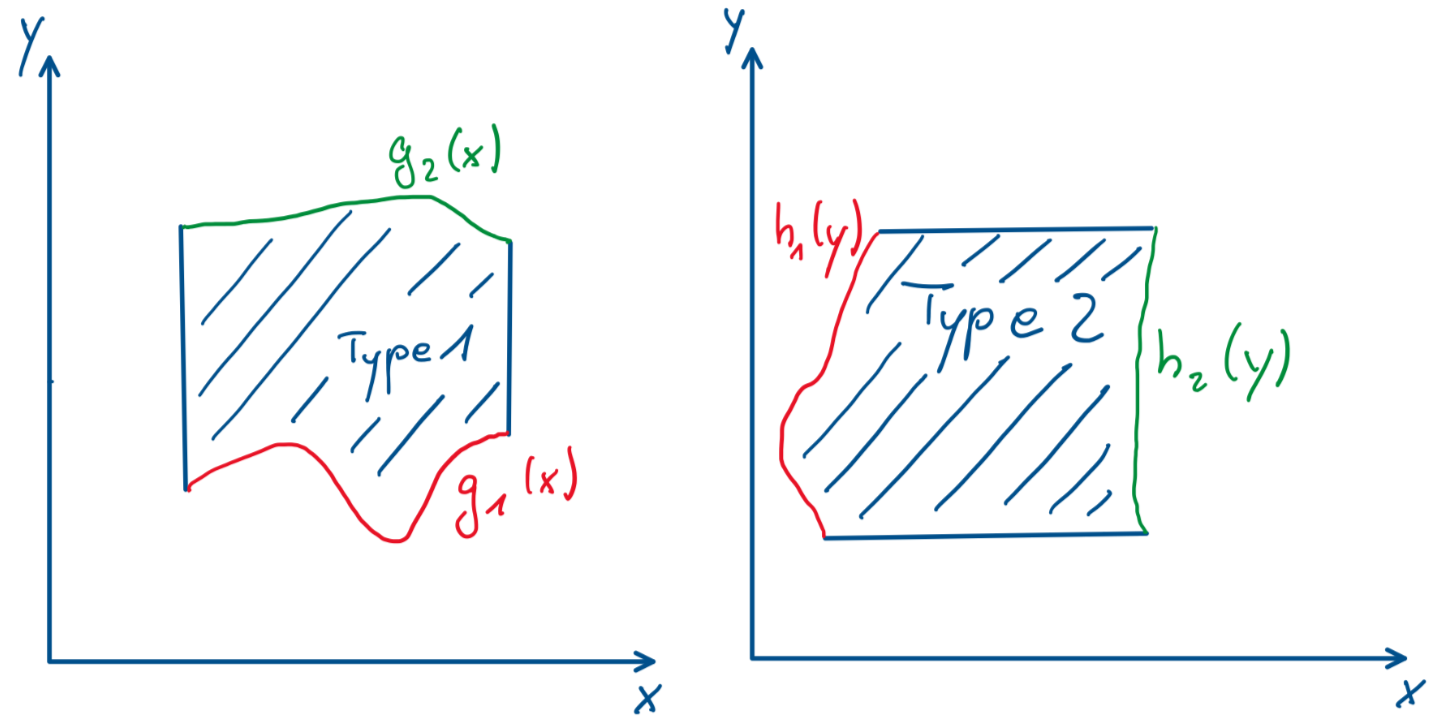
\includegraphics[width=12cm]{Fig/area_types.png}};
  % dekk over det håndskrevne "Type 1" og skriv inn "y-enkelt" i stedet (litt smalere boks, slik at høyre kant av tegningen ikke dekkes)
  \fill[white] ($(areatypesimg.south west)+(2.095,2.774)$) rectangle ($(areatypesimg.south west)+(4.10,3.612)$);
  \node[blue!55!black, font=\Large] at ($(areatypesimg.south west)+(3.0975,3.193)$) {$y$-enkelt};
  % dekk over det håndskrevne "Type 2" og skriv inn "x-enkelt" i stedet (litt smalere boks, slik at høyre kant av tegningen ikke dekkes)
  \fill[white] ($(areatypesimg.south west)+(7.374,2.942)$) rectangle ($(areatypesimg.south west)+(9.30,3.779)$);
  \node[blue!55!black, font=\Large] at ($(areatypesimg.south west)+(8.337,3.360)$) {$x$-enkelt};
\end{tikzpicture}
\caption{$y$-enkle og $x$-enkle områder i planet.}\label{fig:arealtyper}
\end{figure}
\begin{oppsum}{Egenskaper for dobbeltintegraler}
La $D$ være et integrasjonsområde. For alle funksjoner $f,g$ og $c \in \R$ konstant gjelder:
\begin{enumerate}
  \item \[\iint_D (f + cg)\, dA = \iint_D f\, dA + c\iint_D g\, dA \text{  (lineæritet)}\] 
  \item Hvis området deles i to delmengder \( D = D_1 \cup D_2 \)  (slik at $D_1, D_2$ ikke har noen punkter felles), så er:
  \[\iint_D f\, dA = \iint_{D_1} f\, dA + \iint_{D_2} f\, dA\]
\item \textbf{Bytte av integrasjonsrekkefølge.} 
Noen ganger er det nyttig eller nødvendig å bytte integrasjonsrekkefølge for å kunne utføre integrasjonen. Det endrer ikke verdien til integralet, men vi må passe på grensene når vi gjør det. \emph{For å unngå feil bør du tegne en figur.} Her er et (enkelt) \textbf{eksempel} som illustrerer
\[
\int_0^3 \int_{x^2}^9 x^3 e^{y^3} dy\, dx
= \int_0^9 \int_0^{\sqrt{y}} x^3 e^{y^3} dx\, dy
\]
\end{enumerate}
\end{oppsum}

\begin{rem}{Regulære domener}
De fleste områder vi ønsker å integrere over, er verken $x$-enkle eller $y$-enkle. Slike områder kan imidlertid som regel deles opp i endelig mange ikke-overlappende delområder som hver for seg er både $x$-enkle og $y$-enkle. Et slikt område kaller vi et \textbf{regulært domene}.\footnote{Terminologien er hentet fra \cite{Adams}, hvor et slikt område kalles en \emph{regular domain}.} \Cref{fig:regulaertdomene} viser et eksempel: en ringformet region med et hull, som verken er $x$-enkel eller $y$-enkel i seg selv, men som kan deles inn i fire delområder ved hjelp av radielle kutt. Hvert av de fire delområdene er både $x$-enkelt og $y$-enkelt.

Siden dobbeltintegralet er additivt over ikke-overlappende delområder (se egenskap 2 over), kan vi integrere over et regulært domene $D = D_1 \cup D_2 \cup \dots \cup D_n$ ved å summere integralene over hver del:
\[
\iint_D f(x, y)\, dA = \sum_{i=1}^n \iint_{D_i} f(x, y)\, dA,
\]
hvor hvert delintegral $\iint_{D_i} f\, dA$ regnes ut som et $x$-enkelt eller $y$-enkelt integral slik vi har vist over.
\end{rem}

\begin{figure}[ht]
\centering
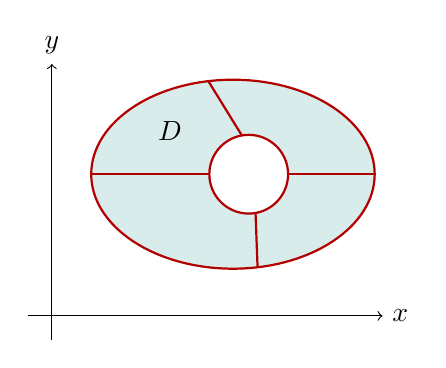
\begin{tikzpicture}[scale=1]
  % koordinatakser
  \draw[->] (-0.3,0) -- (4.2,0) node[right] {$x$};
  \draw[->] (0,-0.3) -- (0,3.2) node[above] {$y$};

  % regulært domene: en ringformet region med et hull
  \begin{scope}
    \clip (2.3,1.8) ellipse (1.8cm and 1.2cm);
    \fill[teal!15] (2.3,1.8) ellipse (1.8cm and 1.2cm);
    \fill[white] (2.5,1.8) circle (0.5cm);
  \end{scope}
  \draw[thick, red!70!black] (2.3,1.8) ellipse (1.8cm and 1.2cm);
  \draw[thick, red!70!black] (2.5,1.8) circle (0.5cm);

  % radielle kutt som deler området i fire x-enkle/y-enkle delområder:
  % høyre (0°) og venstre (180°) rett ut, topp (100°) svakt mot venstre, bunn (280°) svakt mot høyre
  \foreach \ang in {0,100,180,280}{
    \draw[thick, red!70!black]
      ({2.5+0.5*cos(\ang)},{1.8+0.5*sin(\ang)}) --
      ({2.3+1.8*cos(\ang)},{1.8+1.2*sin(\ang)});
  }

  \node at (1.5,2.35) {$D$};
\end{tikzpicture}
\caption{Et regulært domene $D$: en ringformet region med et hull, delt inn i fire delområder ved radielle kutt. Hvert delområde er både $x$-enkelt og $y$-enkelt. Etter \cite{Adams}, Figur 15.12.}
\label{fig:regulaertdomene}
\end{figure}

\begin{eks}{Tenk!}
Parametriser integralet som iterert integral. Er integrasjonsområdet $y$-enkelt eller $x$-enkelt?
\begin{enumerate}
  \item \[
    \iint_D e^{x/y}\, dA, \quad D = \{ (x, y) \mid 1 \leq y \leq 2, \ y \leq x \leq y^3 \}
  \]
  \item \[
    \iint_D (4xy - y^3)\, dA, \quad D =\{(x,y) \mid 1 \leq x \leq  2,  \sqrt{x} \leq  y \leq  x^3\}
  \]
  \item \[
    \iint_D (6x^2 - 40y)\, dA, \quad D = \textrm{trekant med hjørner } (0, 3), (1, 1), (5, 3)
  \]
\end{enumerate}
\end{eks}

\subsection{Flere anvendelser av dobbeltintegraler}
La oss se på noen anvendelser av dobbelintegral.

\subsubsection*{Areal og volum}
Vi kan benytte dobbelintegral både til å beregne volum og areal. 
\begin{oppsum}{Geometrisk tolkning: Areal}
Arealet av et område \( D \) kan finnes ved å integrere konstantfunksjonen $1$:
\[
\text{Areal} = \iint_D 1\cdot dA
\]
Volumet av et område \( D \) kan finnes ved å integrere høyden $z=h(x,y)$ over domenet: 
\[
\text{Volum} = \iint_D h(x,y)\cdot dA
\]
\end{oppsum}

Når vi faktisk skal beregne, deler vi opp i $x$ og/eller $y$-enkle domener. For et $y$-enkelt område kan for eksempel arealdet beregnes som 
\[
\iint_D dA = \int_a^b \int_{g_1(x)}^{g_2(x)} 1\cdot dy\, dx = \int_a^b (g_2(x) - g_1(x))\, dx
\]


\begin{eks}{Bergning av volum}{}
Volumet under flaten \( z = f(x, y) \) og over området \( D \) i \( xy \)-planet.
\[
V = \iint_D f(x, y)\, dA
\]
Finn volumet under \( z = 16xy + 100 \) og over området $D$ i $xy$-planet mellom \( y= x^2 \) og \(y= 8 - x^2 \). Siden $8-x^2=x^2 \Leftrightarrow x=\pm 2$ får vi \( -2 \leq x \leq 2 \) som integrasjonsgrenser. Dermed er 
\begin{align*}
V &= \int_{-2}^{2} \int_{x^2}^{8 - x^2} (16xy + 100) dy\, dx = \int_{-2}^{2}\left[8xy^2+100y\right]_{y=x^2}^{y=8-x^2}\,dx \\ 
&= \int_{-2}^2 512x-128x^3-200x^2+800\, dx = \left[256x^2-32x^4-\frac{200}{3}x^3+800x\right]_{-2}^2 \\ &= \frac{6400}{3}
\end{align*}
\end{eks}

\subsubsection*{Gjennomsnittsverdi}
I analogi med definisjonen av gjennomsnittsverdi for funksjoner av én variabel, gir vi følgende definisjon:
\begin{defn}{Gjennomsnitt av en funksjon}
\emph{Gjennomsnittsverdi} til en funksjon \( f(x,y) \) over området \( D \) er tallet
\[
\bar{f} =
\frac{1}{\text{arealet til } D}
\iint_D f(x,y)\,dA.
\]
Det er ofte svært nyttig å tolke et dobbeltintegral som en gjennomsnittsverdien.
\end{defn}

\begin{eks}{Gjennomsnittsverdi}
Et stort antall punkter \( (x, y) \) velges tilfeldig i trekanten \( T \) med hjørnene \( (0,0) \), \( (1,0) \) og \( (1,1) \). Hvordan kan vi finne gjennomsnittsverdien av \( f(x,y)= x^2 + y^2 \) for disse punktene?

Den gjennomsnittsverdien av \( x^2 + y^2 \) for de tilfeldig valgte punktene vil være gjennomsnittsverdien av funksjonen over trekanten, altså:
\[
\bar{f} = \frac{1}{\text{arealet til } T} \iint_T (x^2 + y^2)\, dA
\]
Trekanten har areal \( \frac{1}{2} \), så ved hjelp av Fubinis teorem:
\[
\bar{f} = 2 \int_0^1 \int_0^x (x^2 + y^2)\, dy\, dx
\]
Vi beregner den indre integralet først:
\[
\int_0^x (x^2 + y^2)\, dy = \int_0^x x^2\, dy + \int_0^x y^2\, dy = x^2 y \big|_0^x + \frac{y^3}{3} \big|_0^x = x^3 + \frac{x^3}{3} = \frac{4x^3}{3}
\]
Så det ytre integralet blir:
\[
\bar{f} = 2 \int_0^1 \frac{4x^3}{3}\, dx = \frac{8}{3} \int_0^1 x^3\, dx = \frac{8}{3} \cdot \frac{1}{4} = \frac{2}{3}
\]
\end{eks}

\subsubsection*{Overflateareal av flater i rommet}
En anvendelsen av dobbeltintegraler er å finne arealet av overflater i tredimensjonale rom når flatene er grafer av funksjoner. Vi skal komme tilbake til slikt når vi har begynt mer ordentlig med vektorkalkulus, men allerede nå kan vi utlede en nyttig formel. La oss se for oss en funksjon 
\[z=f(x,y),\]
se figur~\ref{anv:flateareal}. Dersom vi skal beregne overflatearealet så kan vi se for oss at vi tilnærmer denne overlfaten med små plan $\Delta S_i$ som alle har en prosjeksjon $\Delta A$ ned i $xy$-planet. Ved å summere arealet av alle planene $\Delta S_i$ over hele domenet i $xy$-planet, så kan vi finne det totale overflatearealet. Vi skal nå se hvordan vi kan finne det rette uttrykket for $\Delta S$.

\textbf{Det første steget} er å innse at tangentplanet over ethvert punkt $P$ på grafen kan spennes ut av to tangentvektorer; en som ligger i $xz$-planet og én som ligger i $yz$-planet. Ved å huske tilbake til \Cref{defn:tangentlinje}, kan vi finne uttrykkene for disse tangentvektorene. Der fant vi nemlig at tangentlinjen til grafen $z=f(x)$ i punktet $P=(a,f(a))$ har retningsvektor $\vect t=(1,f'(a))^\top$: øker $x$ med $\Delta x$, øker $z$ langs tangentlinjen med $f'(a)\Delta x$. Tenker vi oss grafen liggende i $xz$-planet i rommet, kan vi skrive den samme retningsvektoren på $\vect i,\vect k$-form:
\(
\vect t = \vect i + f'(a)\vect k,
\)
se \Cref{fig:tangent_1var_motivasjon}.

\begin{figure}[ht]
\centering
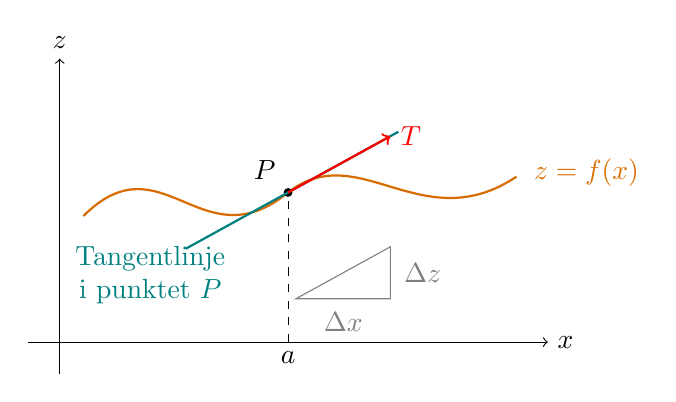
\begin{tikzpicture}[scale=1]
  \draw[->] (-0.4,0) -- (6.2,0) node[right] {$x$};
  \draw[->] (0,-0.4) -- (0,3.6) node[above] {$z$};
  \draw[thick, orange!85!black]
    (0.3,1.6) .. controls (1.3,2.6) and (1.8,1.0) .. (2.9,1.9)
    .. controls (3.8,2.6) and (4.6,1.3) .. (5.8,2.1);
  \node[orange!85!black, right] at (5.9,2.15) {$z=f(x)$};
  \draw[dashed] (2.9,0) node[below] {$a$} -- (2.9,1.9);
  \fill (2.9,1.9) circle (1.6pt);
  \node[above left=1pt] at (2.9,1.9) {$P$};
  \draw[thick, teal] (1.6,1.185) -- (4.3,2.67);
  \node[teal, align=center] at (1.15,0.85) {Tangentlinje\\ i punktet $P$};
  \draw[->, thick, red] (2.9,1.9) -- (4.2,2.615) node[right] {$\vect T$};
  \draw[gray] (3.0,0.55) -- (4.2,0.55) -- (4.2,1.21) -- cycle;
  \node[gray, below] at (3.6,0.5) {$\Delta x$};
  \node[gray, right] at (4.25,0.88) {$\Delta z$};
\end{tikzpicture}
\caption{Tangentlinjen til grafen $z=f(x)$ i punktet $P=(a,f(a))$, med tilhørende tangentvektor $\vect T = \vect i + f'(a)\vect k$. Stigningen $f'(a) = \Delta z/\Delta x$ er forholdet mellom sidene i den lille trekanten.}
\label{fig:tangent_1var_motivasjon}
\end{figure}

\begin{figure}[ht]
\centering
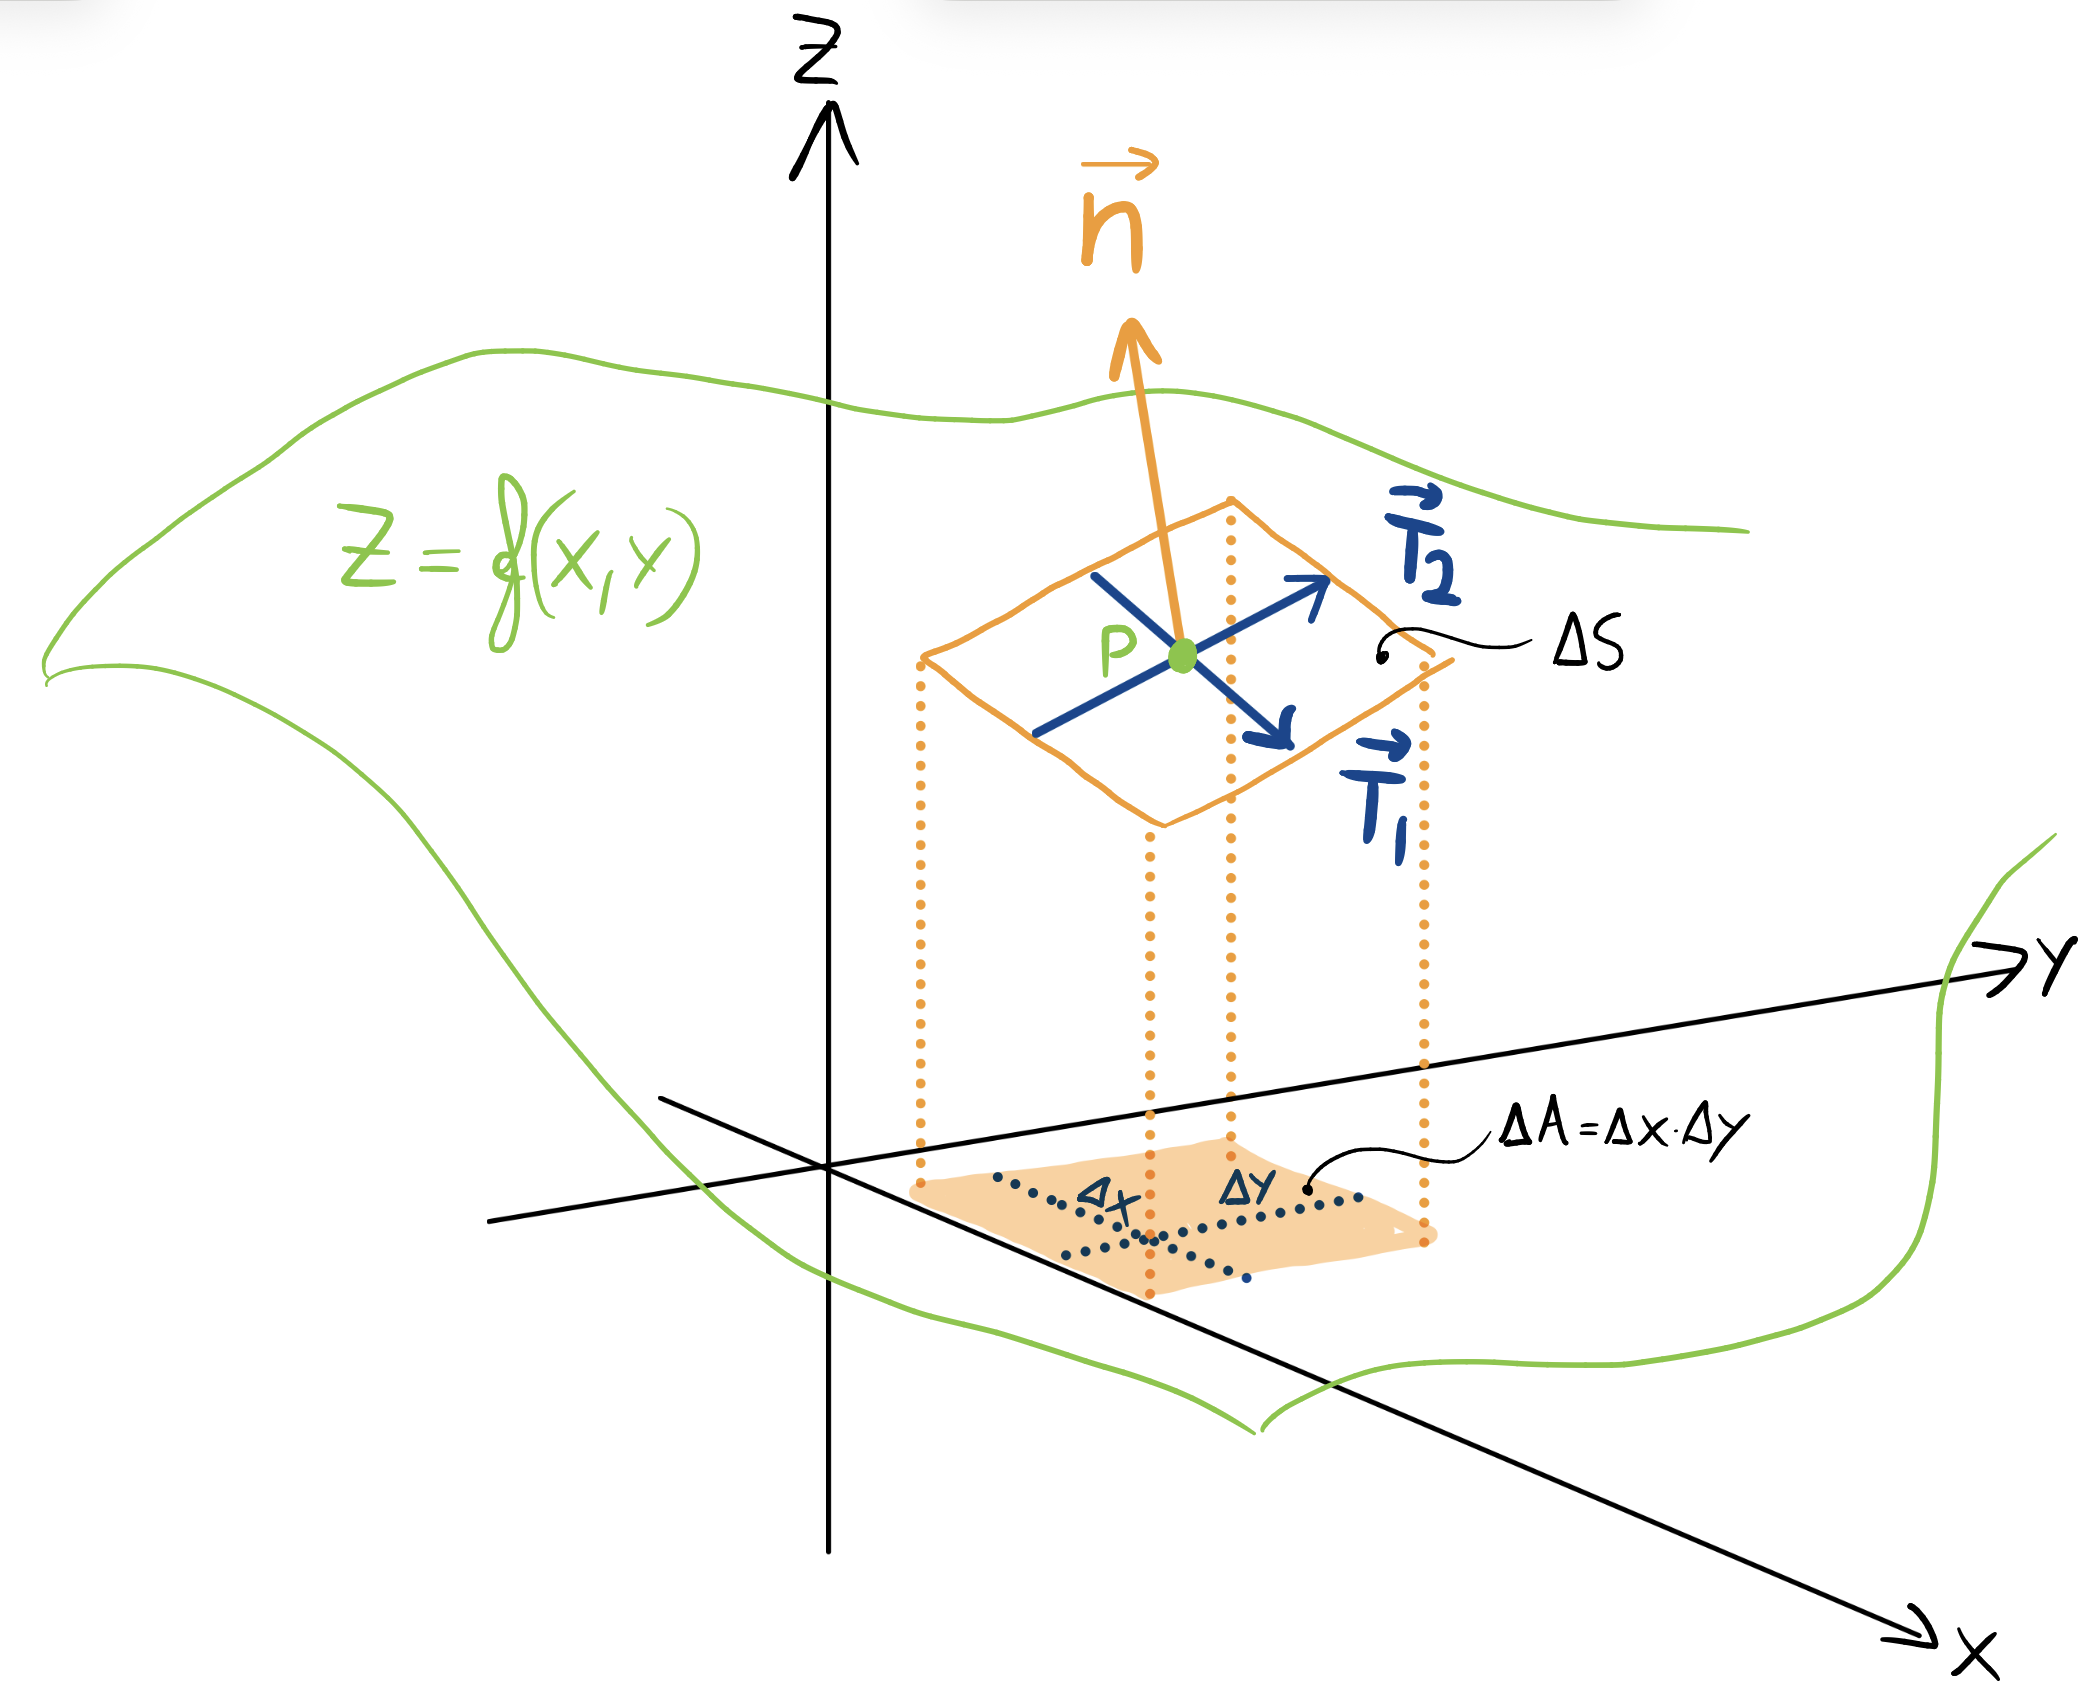
\includegraphics[width=10cm]{Fig/flateelement_tangentplan.png}
\caption{Flateelementet $\Delta S$ i tangentplanet til $z=f(x,y)$ i punktet $P=(a,b,f(a,b))$, utspent av kantvektorene $\vect T_1=\vect i+f_x(a,b)\vect k$ og $\vect T_2=\vect j+f_y(a,b)\vect k$, med normalvektor $\vect n=\vect T_1\times \vect T_2$. $\Delta S$ ligger rett over det lille rektangelet $\Delta A=\Delta x\cdot \Delta y$ i $xy$-planet.}
\label{fig:tangent_2var_motivasjon}
\end{figure}

\textbf{Steg 2: To variabler, to tangentvektorer.} La nå $z=f(x,y)$ være en deriverbar flate, og se på punktet $P=(a,b,f(a,b))$. Vi lager to tangentvektorer til flaten i $P$ ved å holde henholdsvis $y$ og $x$ fast, og bruke resonnementet over på hver av de resulterende kurvene:
\begin{itemize}
  \item Holder vi $y=b$ fast, får vi kurven $z=f(x,b)$ i planet $y=b$. Nøyaktig som over har denne kurven tangentvektor
  \(\vect t_1 = \vect i + f_x(a,b)\vect k.\). Ettersom projeseringen ned på $x$-aksen har størrelse $\Delta x$, kan vi dessuten konkludere at den vektoren som både er tangent til kurven \textit{og} har samme lengde som ene sidekanten til $\Delta S$, må være 
   \[\vect T_1 = \Delta x(\vect i + f_x(a,b)\vect k).\]

  \item Holder vi $x=a$ fast, får vi kurven $z=f(a,y)$ i planet $x=a$, med tangentvektor
  \(\vect t_2 = \vect j + f_y(a,b)\vect k.\) På samme vis vil det gi 
  \[\vect T_2 = \vect j + f_y(a,b)\vect k,\]
  som altså angir den andre lengden i $\Delta S$.
\end{itemize}
Vektorene $\vect T_1$ og $\vect T_2$ ligger begge i tangentplanet til flaten i $P$, og de utgjør sidekantene til  $\Delta S$ (se \Cref{fig:tangent_2var_motivasjon}). 

Fra \Cref{defn:vektorprodukt} i kapittel 0 vet vi at kryssproduktet av $\vect T_1$ og $\vect T_2$ derfor gir arealet av $\Delta S$:
\[
\vect n = \vect T_1 \times \vect T_2 =
\Delta x\Delta y\begin{vmatrix} \vect i & \vect j & \vect k \\ 1 & 0 & f_x(a,b) \\ 0 & 1 & f_y(a,b) \end{vmatrix}
= \Delta A(-f_x(a,b)\,\vect i - f_y(a,b)\,\vect j + \vect k),
\]
med lengde
\[
\lVert \vect n \rVert = \sqrt{f_x(a,b)^2+f_y(a,b)^2+1}\,\Delta A.
\]
Her brukte vi $\Delta A=\Delta x\Delta y$.
Om vi nå lar $\Delta A\to 0$ på den vanlige måten og integrerer så får vi arealet av hele flaten, slik som oppsummert under.



\begin{oppsum}{Arealet av en flate $z=f(x,y)$}
Hvis flaten $S$ i tredimensjonal rom er definert som $z=f(x,y)$ for $(x,y) \in D$ et område i $xy$-planet og $f$ er deriverbar, så kan flatearealet beregnes som 
\begin{align} \label{anv:flateareal}
S = \iint_D \sqrt{\left( \frac{\partial f}{\partial x} \right)^2 + \left( \frac{\partial f}{\partial y} \right)^2 + 1}\, dA
\end{align}
\end{oppsum}
Vi kommer tilbake til tangent- og normalvektorer til flater mer generelt i \Cref{defn:tang_norm}.

\begin{eks}{}
Finn arealet av den delen av planet $3x + 2y + z = 6$ som ligger i første oktant. Vi omskriver likningen til $z = f(x, y)$:
\[
z = 6 - 3x - 2y \Rightarrow f_x = -3, \quad f_y = -2
\]
Området $D$ er trekanten med:
\[
0 \leq x \leq 2, \quad 0 \leq y \leq -\tfrac{3}{2}x + 3
\]
Arealet blir:
\[
S = \iint_D \sqrt{(-3)^2 + (-2)^2 + 1}\, dA = \iint_D \sqrt{14}\, dA = \sqrt{14} \cdot \text{Areal av } D = 3\sqrt{14}
\]
\end{eks}

Vi kommer tilbake til flateintegraler senere.

\section{Polarkoordinater og variabelbytte}\label{sect:polarkoord}

Så langt har vi sett på dobbeltintegraler der området \( D \) enkelt kan beskrives i kartesiske koordinater. I denne seksjonen ser vi på områder som er enklere å beskrive i polarkoordinater, slik som for eksempel disker, ringer eller deler av disse. I det videre vil vi ha nytte av transformasjonen mellom kartesiske koordinater $(x,y)$ og polare koordinater $(r,\theta)$ gitt ved
\begin{align}
    \label{polarTrans}
    &x=r\cos(\theta),\\
    &y=r\sin(\theta).
\end{align}
Her er $r=\sqrt{x^2+y^2}$.

\begin{eks}{Integrasjon over en disk}
\[
\iint_D f(x, y)\, dA, \quad D = \text{disk med radius 1 rundt origo}
\]
I kartesiske koordinater beskrives disken med:
\[
-1 \leq x \leq 1,\quad -\sqrt{1 - x^2} \leq y \leq \sqrt{1 - x^2}
\]
I kartesiske koordinater får vi nå 
\[\iint_D f(x, y)\, dA= \int_{-1}^1 \int_{-\sqrt{1-x^2}}^{\sqrt{1-x^2}} f(x,y) dx \, dy\]
I polarkoordinater kan samme område beskrives mye enklere, som:
\[
0 \leq r \leq 1, \quad 0 \leq \theta \leq 2\pi,\quad
\]
og her ser vi at det er faktisk et rektangel hvor vi kan unngå å bruke kompliserte funksjoner for å beskrive mengden. Integralet blir der 
\[\iint_D f(x, y)\, dA= \int_{0}^1 \int_{0}^{2\pi} f(r\cos(\theta),r\sin(\theta)) r\, d\theta \, dr\]
Integralet har blitt enklere, men det kan se ut som om vi har en skrivefeil: Hvorfor er det en ekstra $r$ i formelen?
\end{eks}
Vi kan ikke bare bytte ut \( dx\, dy \) med \( dr\, d\theta \). For å beregne arealelementet må vi sjekke hvordan arealet til et lite område i polarkoordinater endrer seg. Som \Cref{fig:arealpolar} viser endrer arealet seg annerledes i polarkoordinater enn når vi endrer størrelsen i kartesiske koordinater. Dette gir oss en tilnærming:
\begin{figure}[ht]\centering
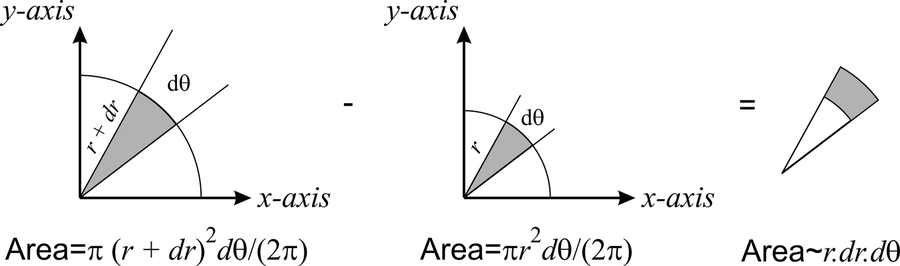
\includegraphics[width=12cm]{Fig/imageedit_7_9308218702.jpg}
\caption{Arealelement i polarkoordinater, (\href{https://creativecommons.org/licenses/by-nc-sa/4.0/}{CC BY-NC-SA 4.0} M. Levitus, \cite{MLon})}\label{fig:arealpolar}
\end{figure}
\[
\Delta A \approx r \Delta r \Delta \theta
\]
som i grensen hvor $\Delta r,\Delta\theta\rightarrow 0$ gir \eqref{areal:polar}. Det riktige arealelementet i polarkoordinater er:

\begin{defn}{Arealelement i polarkoordinater}\label{areal_i_polar}
\begin{align}\label{areal:polar}
dA = r\, dr\, d\theta
\end{align}
\end{defn}
Kanskje husker du at arealelementet i kartesiske koordinater er $dA=dxdy$. En naiv gjetning ville kanskje derfor være at arealelementet i polarkoordinater er $dA=drd\theta$. Men dette er altså feil, noe en også kan se av benevningen (et areal bør ha benevning kvadratmeter; $m^2$). Faktoren $r$ som sniker seg inn kalles \textit{Jacobideterminanten} for polarkoordinater, noe vi snart skal komme tilbake til.

\begin{oppsum}{Konverteringsformler Polarkoordinater}
For å konvertere funksjonen og grensene bruker vi:
\[
x = r \cos \theta,\quad y = r \sin \theta,\quad x^2 + y^2 = r^2.
\]
Dermed blir integralet:
\[
\iint_D f(x, y)\, dA = \int_\alpha^\beta \int_{h_1(\theta)}^{h_2(\theta)} f(r \cos \theta, r \sin \theta) \, r\, dr\, d\theta
\]
Her har vi brukt \eqref{areal:polar} for arealelementet $dA =r\, dr\, d\theta$. Husk at $h_1,h_2$ er funksjoner som er avhengige av integrasjonsområdet $D$, og vi beskrev her faktisk et integrasjonsområde hvor radiusen $r$ er avhengig av vinkelen $\theta$ (det er det vanligste tilfellet).
\end{oppsum}

\begin{eks}{}\mbox{}\\
\begin{minipage}{8cm}
Vi ser på ringen 
\[R= \{(x,y)^\top \colon 1\leq x^2 +y^2\leq 2\}\]
og la integrasjonsområdet være den delen av ringen som ligger mellom vinklene $\frac{\pi}{4}$ og $\frac{5\pi}{4}$.
Bildet til høyre viser mengden $D$ i blå.

Husk at polarkoordinater omdanner en boks i $(r,\theta)$-planet til en ring (eller ball) i det vanlige (kartesiske) $xy$-planet.
\end{minipage}
\begin{minipage}{5cm}
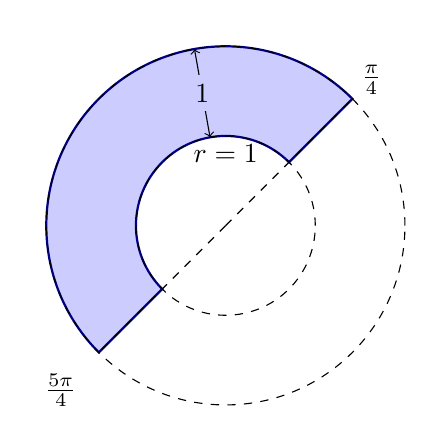
\begin{tikzpicture}
  \begin{axis}[
    axis equal,
    hide axis,
    clip=false,
    xmin=-2.5, xmax=2.5,
    ymin=-2.5, ymax=2.5
  ]

  % Define angular range
  \def\startAngle{45}
  \def\endAngle{225}
  % Outer arc (r = 2)
  \draw[fill=blue!20, draw=blue!50!black, thick]
    ({2*cos(\startAngle)},{2*sin(\startAngle)}) 
    arc[start angle=\startAngle, end angle=\endAngle, radius=2] --
    ({1*cos(\endAngle)},{1*sin(\endAngle)}) 
    arc[start angle=\endAngle, end angle=\startAngle, radius=1] -- cycle;

  \draw[dashed] (0,0) circle (1);
  \draw[dashed] (0,0) circle (2);
  \draw[dashed] (0,0) -- ({2*cos(\startAngle)},{2*sin(\startAngle)});
  \draw[dashed] (0,0) -- ({2*cos(\endAngle)},{2*sin(\endAngle)});

  %: Angle and radius  labels
  \node at ({2.3*cos(45)},{2.3*sin(45)}) {$\frac{\pi}{4}$};
  \node at ({2.6*cos(225)},{2.6*sin(225)}) {$\frac{5\pi}{4}$};
  \node at ({0.6*cos(90)},{0.6*sin(90) + 0.2}) {$r=1$};
  \draw[<->] ({cos(100)},{sin(100)}) -- node[midway, fill=blue!20] {$1$} ({2*cos(100)},{2*sin(100)});
  \end{axis}
\end{tikzpicture}
\end{minipage}
\begin{align*}
 (a) \iint_D xy\, dA &= \int_{\pi/4}^{5\pi/4} \int_1^2 r\cos\theta \cdot r\sin\theta \cdot r \, dr\, d\theta \\
 &= \int_0^{\pi/2} \int_1^2 r^3 \sin(2\theta)\, dr\, d\theta
\\
(b) \iint_D e^{x^2 + y^2} \, dA &=   \int_{\pi/4}^{5\pi/4} \int_1^2 r e^{r^2} \, dr\, d\theta
\end{align*}
\end{eks}

\begin{eks}{}
Finn arealet mellom \( r = 3 + 2\sin\theta \) og \( r = 2 \) for vinkelen \( \theta \in [-\pi/6, 7\pi/6] \):
\[
\iint_D dA = \int_{-\pi/6}^{7\pi/6} \int_2^{3+2\sin\theta} r\, dr\, d\theta
\]
\end{eks}
\begin{figure}[!h]\centering
\tdplotsetmaincoords{70}{110} % viewing angle
\begin{tikzpicture}[tdplot_main_coords]
% Parameters
\def\R{3} % sphere radius
\pgfmathsetmacro{\r}{sqrt(5)}                 % cylinder radius (evaluated number)
\pgfmathsetmacro{\h}{sqrt(\R*\R - \r*\r)}     % z at intersection (=2)

% Axes
\draw[->] (0,0,0) -- (3.5,0,0) node[anchor=north east]{$x$};
\draw[->] (0,0,0) -- (0,3.5,0) node[anchor=north west]{$y$};
\draw[->] (0,0,0) -- (0,0,3.5) node[anchor=south]{$z$};

% Cylinder base in the xy-plane: x^2 + y^2 = 5
\tdplotdrawarc[thick,blue]{(0,0,0)}{\r}{0}{360}{} % base circle

% Cylinder generators up to the sphere
\draw[thick,blue,opacity=0.7] ({\r},0,0) -- ({\r},0,{\h});
\draw[thick,blue,opacity=0.7] ({-\r},0,0) -- ({-\r},0,{\h});
\draw[thick,blue,opacity=0.7] (0,{\r},0) -- (0,{\r},{\h});
\draw[thick,blue,opacity=0.7] (0,{-\r},0) -- (0,{-\r},{\h});

% Intersection circle at z = h where cylinder meets sphere
\tdplotdrawarc[thick,red,dashed]{(0,0,{\h})}{\r}{0}{360}{}

% Upper hemisphere wireframe (a few meridian-like arcs)
\foreach \phi in {0,30,60,90,120,150,180,210,240,270,300,330}{
  \draw[black,thick,opacity=0.35,domain=0:\r,samples=40,smooth,variable=\x]
    plot ({\x*cos(\phi)},{\x*sin(\phi)},{sqrt(\R*\R - \x*\x)});
}

% Labels
%\node at (1.3,1.1,2.2) {$x^2+y^2\le 5,\ z\ge 0$};
%\node at (0.3,-1.3,2.7) {$x^2+y^2+z^2\le 9$};
%\node[red] at (0.2,0.2,{\h+0.2}) {$z=\h$};
\end{tikzpicture} \caption{Volum som skal beregnes i Eksempel 1.11} \label{fig:syl:sph:inter}
\end{figure}

\begin{eks}{Volum under kule og over en sirkel} 
\[\text{Volum under }
z = \sqrt{9 - x^2 - y^2}, \quad \text{ slik at }x^2 + y^2 \leq 5
\]
Volumet vises i \Cref{fig:syl:sph:inter}. I polarkoordinater:
\[
z = \sqrt{9 - r^2}, \quad r \in [0, \sqrt{5}],\ \theta \in [0, 2\pi]
\]
Volum:
\[
V = \int_0^{2\pi} \int_0^{\sqrt{5}} r \sqrt{9 - r^2} \, dr\, d\theta
\]\label{syl:sph:inter}
\end{eks}
\begin{eks}{Volum under plan og over paraboloide}
Beregn volum i figuren
\[
F=\{(x,y,z) \in \R^3 \colon z = 16 - (x^2 + y^2), \quad x^2 + y^2 \leq 16\}
\]
I polarkoordinater:
\[
V = \int_0^{2\pi} \int_0^4 r(16 - r^2) \, dr\, d\theta
\]
\end{eks}
\begin{eks}{Konvertering fra kartesiske til polarkoordinater}
Gitt integral:
\[
\int_{-1}^1 \int_{-\sqrt{1 - x^2}}^0 \cos(x^2 + y^2)\, dy\, dx
\]
Regionen er nedre halvsirkel av radius $1$. I polarkoordinater:
\[
\int_\pi^{2\pi} \int_0^1 r \cos(r^2) \, dr\, d\theta
\]
\end{eks}

Det finnes en annen måte å forstå integraler i andre koordinatsystemer. Det skal vi se nå på for dobbeltintegraler

\subsection*{Variabelbytte}
I tidligere kurs har vi lært at vanlige integraler kan beregnes ved hjelp av substitusjonsregelen:
\[
\int_a^b f(g(x)) g'(x)\, dx = \int_c^d f(u)\, du
\]
Dette var et eksempel på å endre integrasjonsvariabel. Nå ønsker vi å gjøre noe tilsvarende for dobbeltintegraler.

\begin{defn}{Transformasjoner}
En \emph{transformasjon}\footnote{Teknisk sett ønsker vi vanligvis å ha en en-til-en (=bijektiv) funksjon som omdanner et område til et annet. I vanlig ingeniørpraksis skal vi ikke snakke så mye om disse tekniske detaljene.} er et sett av ligninger som endrer variablene:
\[
x = g(u, v), \quad y = h(u, v)\quad \text{eller kortere } x=x(u,v), y=y(u,v)
\]
Her antar vi at funksjonene $g,h$ er minst kontinuerlige (men i praksis krever vi at de er kontinuerlig deriverbare). Området $R$ i $xy$-planet transformeres til et område $S$ i $uv$-planet. 
\end{defn}

\begin{defn}{Jacobideterminant og arealelementet}
For en transformasjon $x = g(u, v), y = h(u, v)$ defineres Jacobideterminant\footnote{Som vanlig betyr strek ved siden av en matrise at vi regner determinanten!} som:
\[
\frac{\partial(x, y)}{\partial(u, v)} = \begin{vmatrix} \frac{\partial x}{\partial u} & \frac{\partial x}{\partial v} \\ \frac{\partial y}{\partial u} & \frac{\partial y}{\partial v} \end{vmatrix}
\]
\end{defn}
Nå får vi en generalisering av substitusjonsformelen 
\begin{oppsum}{Variabelbytte for dobbeltintegraler}
La $x=g(u,v),y=h(u,v)$ være en transformasjon. Så gjelder formelen for variabelbytte for dobbeltintegraler:
\begin{align}\label{eq:variabelbytte}
\iint_R f(x, y)\, dA = \iint_S f(g(u, v), h(u, v))\frac{\partial(x, y)}{\partial(u, v)}\, du\, dv
\end{align}
\end{oppsum}

\begin{eks}{Polarkoordinater}
Polarkoordinater er gitt ved transformasjonen
\[
x = r\cos\theta, \quad y = r\sin\theta
\]
Hvis vi regner ut Jacobideterminanten så får vi:
\[
\frac{\partial(x, y)}{\partial(r, \theta)} = r \Rightarrow dA = r\, dr\, d\theta
\]
Setter vi det inn får vi den kjente formelen for areal i polarkoordinater, \Cref{areal_i_polar}.
\end{eks}

\begin{eks}{Anvendelse: Areal av en ellipse}
Lag en transformasjon for å finne arealet av ellipsen \( E \) gitt ved
\[
\frac{x^2}{a^2} + \frac{y^2}{b^2} < 1
\]
Vi bruker transformasjonen \( x = au \), \( y = bv \). Da er ellipsen \( E \) bildet av disken \( D \) gitt ved \( u^2 + v^2 < 1 \), ved en én-til-én-transformasjon. Anta at \( a > 0 \) og \( b > 0 \). Da har vi:
\[
dx\,dy = \frac{\partial(x,y)}{\partial(u,v)} \, du\,dv
\quad \text{ hvor } \frac{\partial(x,y)}{\partial(u,v)} =
\left|
\begin{array}{cc}
\frac{\partial x}{\partial u} & \frac{\partial x}{\partial v} \\
\frac{\partial y}{\partial u} & \frac{\partial y}{\partial v}
\end{array}
\right|
=
\left|
\begin{array}{cc}
a & 0 \\
0 & b
\end{array}
\right|
= ab
\]
Derfor er arealet av \( E \) gitt ved:
\[
\text{Areal}(E) = \iint_E dx\,dy = \iint_D ab\,du\,dv = ab \iint_D du\,dv = ab \cdot (\text{arealet av } D) = ab \cdot \pi = \pi ab
\]
\end{eks}
Ofte vil man bruke formelen for variabelbytte for å transformere integrasjonsområdet til et rektangel, slik at iterasjon blir enklere. Som følgende eksempel viser, innebærer dette vanligvis at man må definere den inverse transformasjonen (altså \( u \) og \( v \) som funksjoner av \( x \) og \( y \)). Husk at inverse transformasjoner har inverse Jacobideterminanter.

\begin{eks}{}\mbox{}\\
\begin{minipage}{8cm}Finn arealet av området $D$ i planet som er avgrenset av de fire parablene  
\( y = x^2 \), \( y = 2x^2 \), \( x = y^2 \), og \( x = 3y^2 \).
La
\[
u = \frac{y}{x^2}, \quad v = \frac{x}{y^2}
\]
Da tilsvarer området \( D \) rektangelet \( R \) i \( uv \)-planet, gitt ved  
\( 1 \leq u \leq 2 \) og \( 1 \leq v \leq 3 \).
\begin{align*}
\frac{\partial(u, v)}{\partial(x, y)} &=
\begin{vmatrix}
\frac{\partial u}{\partial x} & \frac{\partial u}{\partial y} \\
\frac{\partial v}{\partial x} & \frac{\partial v}{\partial y}
\end{vmatrix} = \begin{vmatrix}
\frac{-2y}{x^3} & \frac{1}{x^2} \\
\frac{1}{y^2} & \frac{-2x}{y^3}
\end{vmatrix}
= \frac{3}{x^2y^2} \\ &= 3\frac{\color{red} x^2 y^2}{y^{\color{red}4}x^{\color{red}4}} = 3u^2v^2
\end{align*}
\end{minipage}
\label{ex:parabolas}
\begin{minipage}{6cm}
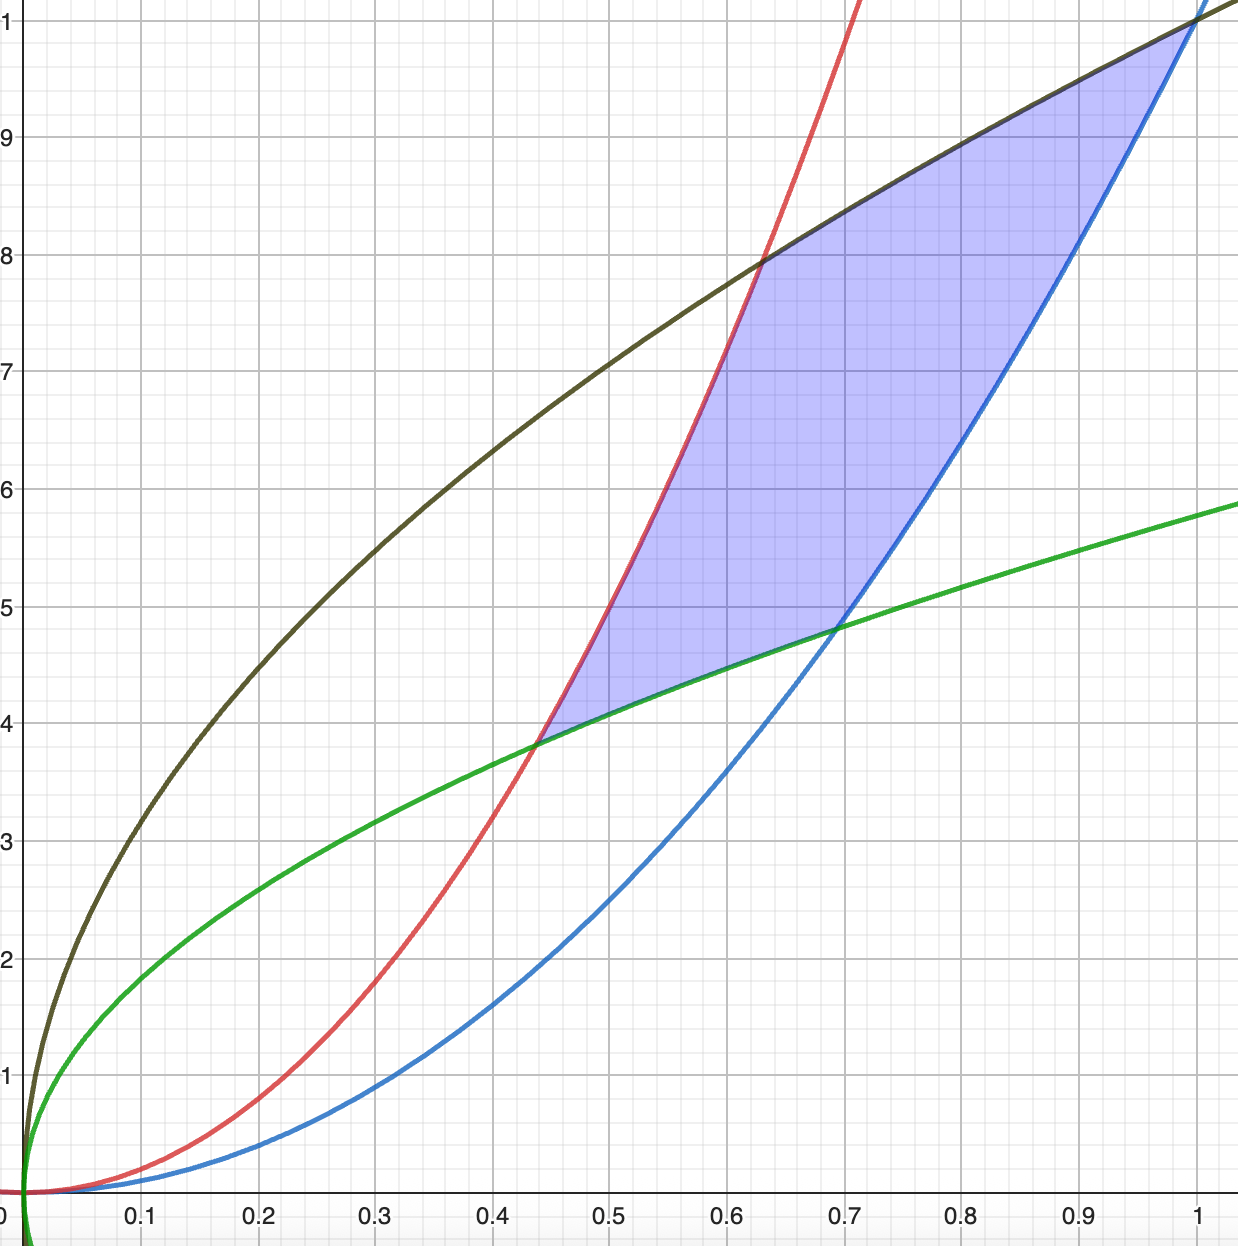
\includegraphics[width=6cm]{Fig/Area_parabolas.png}
\end{minipage}

så følger det at
\[
\frac{\partial(x, y)}{\partial(u, v)} = \frac{1}{\frac{\partial(u, v)}{\partial(x, y)}} = \frac{\partial(x, y)}{\partial(u, v)} = \frac{1}{3u^2v^2}
\]
Derfor er arealet av \( D \) gitt ved
\[
\text{Areal}(D) = \iint_D dx\,dy = \iint_R  \frac{\partial(x, y)}{\partial(u, v)}  du\,dv = \iint_R \frac{1}{3u^2v^2} du\,dv
\]
Vi beregner integralet:
\[
\iint_R \frac{1}{3u^2v^2} du\,dv = \frac{1}{3} \int_1^2 \frac{1}{u^2} du \int_1^3 \frac{1}{v^2} dv = \frac{1}{3} \left[ -\frac{1}{u} \right]_1^2 \left[ -\frac{1}{v} \right]_1^3 = \frac{1}{3} \cdot \left( \frac{1}{1} - \frac{1}{2} \right) \cdot \left( \frac{1}{1} - \frac{1}{3} \right)
\]
\[
= \frac{1}{3} \cdot \frac{1}{2} \cdot \frac{2}{3} = \frac{1}{9}
\]
\end{eks}

\section{Numerisk beregning av dobbeltintegraler}\label{sect:numdobbelt}
Grunnleggende er problemet å beregne 
\[\iint_R f(x,y) dA\]
for en gitt funksjon over et rektangle $R=[a,b]\times [c,d]$. Husk at vi kan forstå integralet som beregning av en (orientert) volum
\begin{figure}[ht]\centering
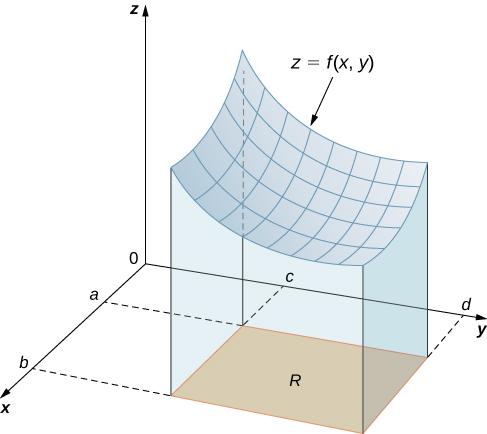
\includegraphics[width=8cm]{Fig/surf3D_rect1.jpg}
\caption{Integralet som volum under en flate. Kilde: \cite{SaH}, \href{https://creativecommons.org/licenses/by-nc-sa/4.0/}{CC BY-NC-SA 4.0}}
\end{figure}
I definisjonen av dobbeltintegralet har vi sett at den er grenseverdien til noen dobbelte Riemann summer. Som i 1D lager vi en approksimasjon ved å dele inn integrasjonsområdet i småbiter og deretter beregner vi summen av volumet over hver liten boks i integrasjonsområdet. Sjekk \Cref{fig:litenbox}.
\begin{figure}[ht]\centering
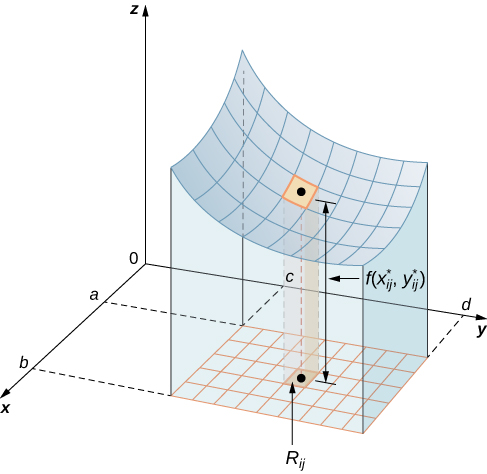
\includegraphics[width=8cm]{Fig/surf_box.jpg}
\caption{Elementer i Riemann summer tilsvarer (orientert) volum over en liten boks. Kilde: \cite{SaH}: \href{https://creativecommons.org/licenses/by-nc-sa/4.0/}{CC BY-NC-SA 4.0}.}\label{fig:litenbox}
\end{figure}
Det vi må dermed implementere for våre numeriske beregninger er en automatisert måte å lage slike oppdelinger av integrasjonsområdet på. Vi illustrerer det i \Cref{dobbelt:mesh}.
\begin{figure}[ht]\centering
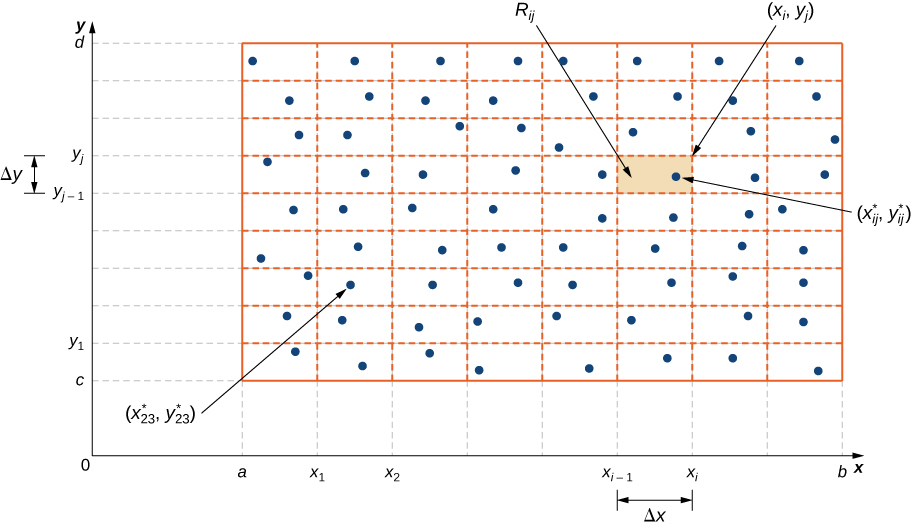
\includegraphics[width=10cm]{Fig/mesh_surf.jpg}
\caption{Gitter for integrasjon. Kilde: \cite{SaH}:\href{https://creativecommons.org/licenses/by-nc-sa/4.0/}{CC BY-NC-SA 4.0}.}\label{dobbelt:mesh}
\end{figure}


Python-kommandoer som hjelper med det finnes i NumPy-pakken:
\begin{lst}{}
import numpy as np

np.meshgrid

np.mgrid
\end{lst}
Tilsvarende finnes det kommandoer i SciPy-pakken:
\begin{lst}{}
import scipy as sp

sp.integrate.dblquad
\end{lst}

Ved Jupyter Hub finner dere to notatbøker hvor vi skal se på
\begin{itemize}
\item integrasjon ved hjelp av gittermetoden og Scipy
\item numerisk integrasjon av diskret data.
\end{itemize}
\section{Trippelintegral}\label{sect:trippelint}

Vi har definert hvordan man integrerer over områder i todimensjonalt rom. Det er nå enkelt å utvide til tre dimensjoner og integrere over områder $E \subseteq \R^3$. For dette definerer man \emph{trippelintegral}:
\[
\iiint_E f(x, y, z)\, dV := \lim \sum_{i=1}^{l} \sum_{j=1}^{m} \sum_{k=1}^{n} f(x^{*}_{ijk}, y^{*}_{ijk}, z^{*}_{ijk}) \, \Delta x \, \Delta y \, \Delta z.
\]
Egentlig måtte man nå sjekke betydningen av grenseverdien som gir trippelintegralet (det vi allerede har gjort for dobbeltintegraler). Vi skal se på det litt senere i \Cref{sect:num_met1}. I stedet starter vi med enkle integrasjonsområder som er bokser. En variant av Fubinis teorem \ref{thm:fubini} gjelder her, og dermed kan vi i stedet for grenseverdidefinisjonen se på trippelintegralet ved hjelp av itererte integraler:

\begin{defn}{Trippelintegral via itererte integraler}
For en boks $B = [a,b] \times [c,d] \times [r,s]$, er integralet:
\[
\iiint_B f(x, y, z)\, dV := \int_r^s \int_c^d \int_a^b f(x, y, z)\, dx\, dy\, dz
\]
Rekkefølgen på integrasjon kan velges fritt avhengig av funksjon og grenser.
\end{defn}

\begin{eks}{} Beregn 
\[
\iiint_B 8xyz\, dV \quad \text{hvor } B = [2, 3] \times [1, 2] \times [0, 1]
\]
Vi bruker itererte integraler
\begin{align*}
\iiint_B 8xyz\, dV&=\int_0^1 \int_1^2 \int_2^3 8xyz \, dx\,dy\,dz = \int_0^1 \int_1^2 4yz[x^2]_2^3\, dy\, dz = \int_0^1 2z[y^2]_1^2 (9-4)\,dz\\
&= 5\cdot 3 \cdot [z^2]_0^1 =15
\end{align*}
\end{eks}

\begin{defn}{Generelle områder – $z$-enkle områder}
Vi definerer et $z$\emph{-enkelt område} $E$ slik:\footnote{Analogt med dobbeltintegraler (se \Cref{sect:dobbelint}) omtales disse tre områdetypene i andre kilder også som \emph{Type 1}, \emph{Type 2} og \emph{Type 3} (eller \emph{Type I}, \emph{Type II}, \emph{Type III}). Vi bruker gjennomgående $z$-enkelt, $x$-enkelt og $y$-enkelt i dette kompendiet.}
\[
E = \{(x, y, z) \mid (x, y) \in D,\, u_1(x, y) \leq z \leq u_2(x, y)\}
\]
Her er $(x, y) \in D$ et område i $xy$-planet, og integralet evalueres som:
\[
\iiint_E f(x, y, z)\, dV = \iint_D \left[\int_{u_1(x,y)}^{u_2(x,y)} f(x, y, z)\, dz\right]\, dA
\]
\end{defn}
\begin{eks}{}%\mbox{}
\begin{minipage}{6cm}
Hvis \( T \) er tetraederet med hjørner \((0, 0, 0)\), \((1, 0, 0)\), \((0, 1, 0)\), og \((0, 0, 1)\), finn verdien av integralet
\[
\iiint_T y \, dV.
\]
Tetraederet er vist i bildet til høyre. Det er et $z$-enkelt område. Et snitt i planet normalt på \(x\)-aksen i posisjon \(x\) er trekanten \(T(x)\), vist i figuren. Her er \(x\) konstant og \(y\) og \(z\) er variable i snittet. Dobbeltintegralet av \(y\) over \(T(x)\) er en funksjon av \(x\).
\end{minipage} 
\begin{minipage}{8cm}
\tdplotsetmaincoords{70}{120}
\begin{tikzpicture}[tdplot_main_coords, scale=5]
  % Define points
  \coordinate (O) at (0,0,0);
  \coordinate (A) at (1,0,0);
  \coordinate (B) at (0,1,0);
  \coordinate (C) at (0,0,1);
  \coordinate (X) at (0.4,0,0);
  \coordinate (Y) at (0.4,0.6,0);
  \coordinate (Z) at (0.4,0,0.6);

  % Draw coordinate axes
  \draw[->, thick] (O) -- (1.1,0,0) node[below left] {$x$};
  \draw[->, thick] (O) -- (0,1.1,0) node[below right] {$y$};
  \draw[->, thick] (O) -- (0,0,1.1) node[left] {$z$};

  % Draw tetrahedron edges
  \draw[thick] (O) -- (A) -- (B) -- cycle;
  \draw[thick] (O) -- (B);
  \draw[thick] (O) -- (C);
  \draw[thick] (A) -- (C);
  \draw[thick] (B) -- (C);

  % Shaded triangle T(x)
  \filldraw[fill=cyan!20, draw=blue, thick, opacity=0.6] (X) -- (Y) -- (Z) -- cycle;

  % Vertical red line from base to z
  \draw[red, thick] (Y) -- (Z);

  % Labels
  \node at (0.5,0.175,0.25) {$T(x)$};
  \node at (0.15,0.5,0.3) {$T$};
  \node at (0.1,0.75,0.75) {$z = 1 - x - y$};
  \node at (0.55,1,0) {\small $y = 1 - x,\ z = 0$};

  % Axes ticks
  \node at (1,0,-.05) {\small $1$};
  \node at (0,1,0.1) {\small $1$};
  \node at (-0.1,0,1) {\small $1$};
\end{tikzpicture}
\end{minipage}

 Vi evaluerer integralet ved å integrere først i \(z\)-retningen, deretter i \(y\)-retningen, som antydet i figuren.
\begin{align*}
\iint_{T(x)} y \, dA &= \int_0^{1 - x} \int_0^{1 - x - y} y \, dz \, dy = \int_0^{1 - x} y(1 - x - y) \, dy\\
&= \int_0^{1 - x} \left[y(1 - x) - y^2\right] \, dy 
= (1 - x) \int_0^{1 - x} y \, dy - \int_0^{1 - x} y^2 \, dy\\
&= = \frac{1}{2}(1 - x)^3 - \frac{1}{3}(1 - x)^3 
= \left( \frac{1}{2} - \frac{1}{3} \right)(1 - x)^3 
= \frac{1}{6}(1 - x)^3
\end{align*}
Til slutt integrerer vi med hensyn på \(x\):
\[
\iiint_T y dV = \int_0^1 \iint_{T(x)} y dA= \int_0^1 \frac{1}{6}(1 - x)^3 \, dx = \frac{1}{6} \int_0^1 (1 - x)^3 \, dx
= \frac{1}{6} \cdot \frac{1}{4} = \frac{1}{24}
\]
I beregningen ovenfor utførte vi integrasjon i to trinn for å tydelig vise fremgangsmåten. I praksis utføres trippelintegraler i ett trinn, uten at dobbeltintegralet over snittet nevnes eksplisitt.
\label{ex:tetrahedron}
\end{eks}

\begin{defn}{$x$-enkle og $y$-enkle områder}
Et $x$\emph{-enkelt område} $E$ defineres som:
\[
E = \{(x, y, z) \mid (y, z) \in D,\, u_1(y, z) \leq x \leq u_2(y, z)\}
\]
For et slikt område er integralet definert som:
\[
\iiint_E f(x, y, z)\, dV = \iint_D \left[\int_{u_1(y,z)}^{u_2(y,z)} f(x, y, z)\, dx\right]\, dA
\]
Et $y$\emph{-enkelt område} $E$ defineres som:
\[
E = \{(x, y, z) \mid (x, z) \in D,\, u_1(x, z) \leq y \leq u_2(x, z)\}
\]
For disse områder definerer man integralet slik 
\[
\iiint_E f(x, y, z)\, dV = \iint_D \left[\int_{u_1(x,z)}^{u_2(x,z)} f(x, y, z)\, dy\right]\, dA
\]
\end{defn}

\begin{rem}{OBS: Variable grenser i tripleintegraler}
Merk at området $D$ vi har sett på i de $x$-, $y$- og $z$-enkle integrasjonsområdene, i hvilket som helst av planene, kan være $y$-enkelt eller $x$-enkelt som beskrevet tidligere.
Hvis $D$ i $xy$-planet er $y$-enkelt, så gjelder
\[
E = \{(x,y,z) \mid a \leq x \leq b, \; g_{1}(x) \leq y \leq g_{2}(x), \; u_{1}(x,y) \leq z \leq u_{2}(x,y) \}.
\]
I $xyz$-rommet har vi en komplisert form $E$ med toppflate $z = u_{2}(x,y)$ og bunnflate $z = u_{1}(x,y)$. Bunnen projiseres ned på $xy$-planet som området $D$ med grensene 
\[
x = a, \quad x = b, \quad y = g_{1}(x), \quad y = g_{2}(x).
\]
Da er begge grenser i de indre integralene avhengige av de andre variablene, og trippelintegralet er
\[
\iiint_{E} f(x,y,z) \, dV 
= \int_{a}^{b} \int_{g_{1}(x)}^{g_{2}(x)} \int_{u_{1}(x,y)}^{u_{2}(x,y)} 
f(x,y,z) \, dz \, dy \, dx.
\]
\end{rem}


\begin{eks}{}
Evaluer:
\[
\iiint_E \sqrt{3x^2 + 3z^2}\, dV \quad \text{hvor } E \text{ er fastlegemet begrenset av } y = 2x^2 + 2z^2 \text{ og } y = 8
\]
\end{eks}

\begin{rem}{Tolkning som Volum} Volumet av et område $E \subseteq \R^3$ er gitt ved:
\[
V = \iiint_E 1\, dV
\]
\end{rem}

\subsection*{Anvendelse: Momenter og massens tyngdepunkt}

Tyngdepunktet til et stivt legeme er det punktet (fast i kroppen) hvor kroppen kan støttes slik at den, i et konstant gravitasjonsfelt, ikke vil oppleve noen ubalanserte dreiemomenter som får den til å rotere.

Dreiemomentene som virker på et masseelement \( dm \) i kroppen kan uttrykkes ved momentene til \( dm \) om de tre koordinatplanene. Vi antar at kroppen fyller et område \( R \) i tredimensjonalt rom og har en kontinuerlig tetthet \( \delta(x, y, z) \), så er masseelementet
$
dm = \delta(x, y, z) \, dV,
$
som opptar et volumelement \( dV \). Total masse til kroppen er dermed gitt som 
\[m=\iiint \delta(x,y,z) dV.\]
Vi sier at kroppen har momentene
$(x - x_0) \, dm, \quad (y - y_0) \, dm, \quad (z - z_0) \, dm
$ om planene\footnote{Vi anbefaler å skissere betydningen av $x-x_0$ og hvorfor mengden av $(x,y,z)$ slik at $x=x_0$ danner et plan i det tredimensjonale rommet!} \( x = x_0 \), \( y = y_0 \), og \( z = z_0 \), henholdsvis.
Dermed er de totale momentene til kroppen om disse tre planene:
\begin{align*}
M_{x=x_0} =\iiint_R (x - x_0)\delta(x, y, z)\,dV = M_{x=0} - x_0 m,\\
M_{y=y_0} =\iiint_R (y - y_0)\delta(x, y, z)\,dV = M_{y=0} - y_0 m,\\
M_{z=z_0} =\iiint_R (z - z_0)\delta(x, y, z)\,dV = M_{z=0} - z_0 m.
\end{align*}

Der $m = \iiint_R \delta\, dV$ er massen til kroppen, og $M_{x = 0}, \quad M_{y = 0}, \quad M_{z = 0}$ er momentene om koordinatplanene \( x = 0 \), \( y = 0 \), og \( z = 0 \), henholdsvis.

Tyngdepunktet \( P = (x, y, z) \) til kroppen er det punktet $\hat{P} = (\hat{x},\hat{y},\hat{z})$ for hvilket
\[
M_{x=\hat{x}} = 0, \quad M_{y=\hat{y}} = 0, \quad M_{z=\hat{z}} = 0.
\]

\begin{defn}{Tyngdepunkt}
Tyngdepunktet til et legeme som fyller et område \( R \) i det tredimensjonale rommet og har en kontinuerlig tetthet \( \delta(x, y, z) \) (masseenhet per volumenhet) er punktet \( (\hat{x}, \hat{y}, \hat{z}) \) med koordinater gitt ved:
\begin{align*}
\hat{x} = \frac{1}{m} \iiint_R x \, \delta(x, y, z)\, dV, \quad
\hat{y} = \frac{1}{m} \iiint_R y \, \delta(x, y, z)\, dV, \quad
\hat{z} = \frac{1}{m} \iiint_R z \, \delta(x, y, z)\, dV\\
\text{ hvor den totale massen til kroppen er beregnet som }m = \iiint_R \delta dV
\end{align*}
\end{defn}
Disse formlene kan kombineres til en enkelt vektorformel for posisjonsvektoren \( \vect{r} = x\vect{i} + y\vect{j} + z\vect{k} \) til tyngdepunktet:
\[
\vect{r} = \frac{M_{x=0}\vect{i}+M_{y=0}\vect{j}+M_{z=0}\vect{k}}{m}=\frac{1}{m} \iiint_R \delta\mathbf{r}(x, y, z)\, dV
\]

hvor integralet av den vektorverdige funksjonen \( \delta \mathbf{r} \) betyr vektoren der komponentene er integralene til komponentene av \( \delta \mathbf{r} \).

\begin{rem}{}
Tilsvarende uttrykk gjelder for massedistribusjoner over områder i planet eller over intervaller på en linje. Vi bruker da arealtetthet eller linjetetthet, og dobbeltintegral eller de vanlige bestemte integraler.

Hvis tettheten er konstant, kanselleres den ut i uttrykkene for tyngdepunktet. I dette tilfellet er tyngdepunktet en geometrisk egenskap ved området \( R \), og kalles da \emph{sentroidet} eller \emph{tyngdepunktet} til området. 
\end{rem}

\begin{eks}{}
Beregn sentroidet av tetraederet $T$ (fra \Cref{ex:tetrahedron}) som ligger mellom koordinatplanene og planet gitt som $x+y+z=1$.

Tettheten er konstant, så vi antar at tettheten er lik $1$. Massen til $T$ er dermed lik volumet\footnote{Husk at en tetraeder er et spesielt tilfelle av en pyramide. \href{https://no.wikipedia.org/wiki/Pyramide}{Wikipedia} minner oss at dens volum er en tredjedel av grunnflaten ganger høyden. Her er grunnflaten en rettvinklet trekant slik at $A=1/2$, og høyden er $1$. Hvis man ikke liker det, kan man også regne ut et trippelintegral.}, dvs. $m=V=\frac{1}{6}$. Symmetrien i problemet gjør at sentroiden $(\overline{x},\overline{y},\overline{z})$ oppfyller $\overline{x}=\overline{y}=\overline{z}$. Det er dermed nok at vi beregner 
\[\overline{y}=\frac{M_{y=0}}{m} = 6 \cdot \iiint_T y dV = 6 \cdot \frac{1}{24} =  \frac{1}{4}\]
(se \Cref{ex:tetrahedron} for regning!). Dermed er sentroid her $(\tfrac{1}{4},\tfrac{1}{4},\tfrac{1}{4})$.
\end{eks}

\section{Trippelintegraler i andre koordinater}\label{sect:trippelint_andre}
Som i todimensjonalt rom er det ofte enklere å uttrykke noen integraler ved hjelp av andre koordinater. Det gjelder igjen en versjon av variabelbytteformelen \Cref{eq:variabelbytte} for trippelintegraler. Vi definerer transformasjoner som en spesiell type funksjoner (igjen går vi her ikke så nøye inn på detaljene). Så hvis \[x=x(u,v,w), \quad y=y(u,v,w), \quad z=z(u,v,w)\]
er en transformasjon, knytter vi volumelementene sammen ved bruk av determinanten til Jacobi-matrisen. For volumet er det da
\begin{align}\label{eq:volum_variablebytte}
dV = dx\, dy\, dz = \frac{\partial (x,y,z)}{\partial (u,v,w)} du\, dv\, dw. \\ 
\text{hvor } \frac{\partial(x,y,z)}{\partial(u,v,w)}:= \begin{vmatrix} \frac{\partial x}{\partial u} & \frac{\partial x}{\partial v} & \frac{\partial x}{\partial w} \\ \frac{\partial y}{\partial u} & \frac{\partial y}{\partial v} & \frac{\partial y}{\partial w} \\ \frac{\partial z}{\partial u} & \frac{\partial z}{\partial v} & \frac{\partial z}{\partial w}\end{vmatrix}\notag\end{align}
Hvis vi har et trippelintegral av en funksjon, så betyr det at vi må multiplisere funksjonen med determinanten for å integrere i de andre koordinatene. Det er akkurat \eqref{eq:variabelbytte} for trippelintegraler!
\begin{oppsum}{Variabelbytte for trippelintegraler}
La $x=x(u,v,w),y=y(u,v,w), z=z(u,v,w)$ være en transformasjon. Så gjelder formelen for variabelbytte for trippelintegraler:
\begin{align*}
\iiint_R f(x, y,z)\, dV = \iiint_S f(x(u, v,w), y(u, v,w), z(u,v,w))\frac{\partial(x, y,z)}{\partial(u, v,w)}\, du\, dv\, dw
\end{align*}
\end{oppsum}
Som et første eksempel skal vi se på trippelintegraler i sylindriske koordinater. 
\subsection{Trippelintegraler i sylindriske koordinater}
Husk at sylindriske koordinater bare er en utvidelse av polarkoordinater til tre dimensjoner (se også \Cref{sect:koordinater}).
\begin{figure}[ht]\begin{center}
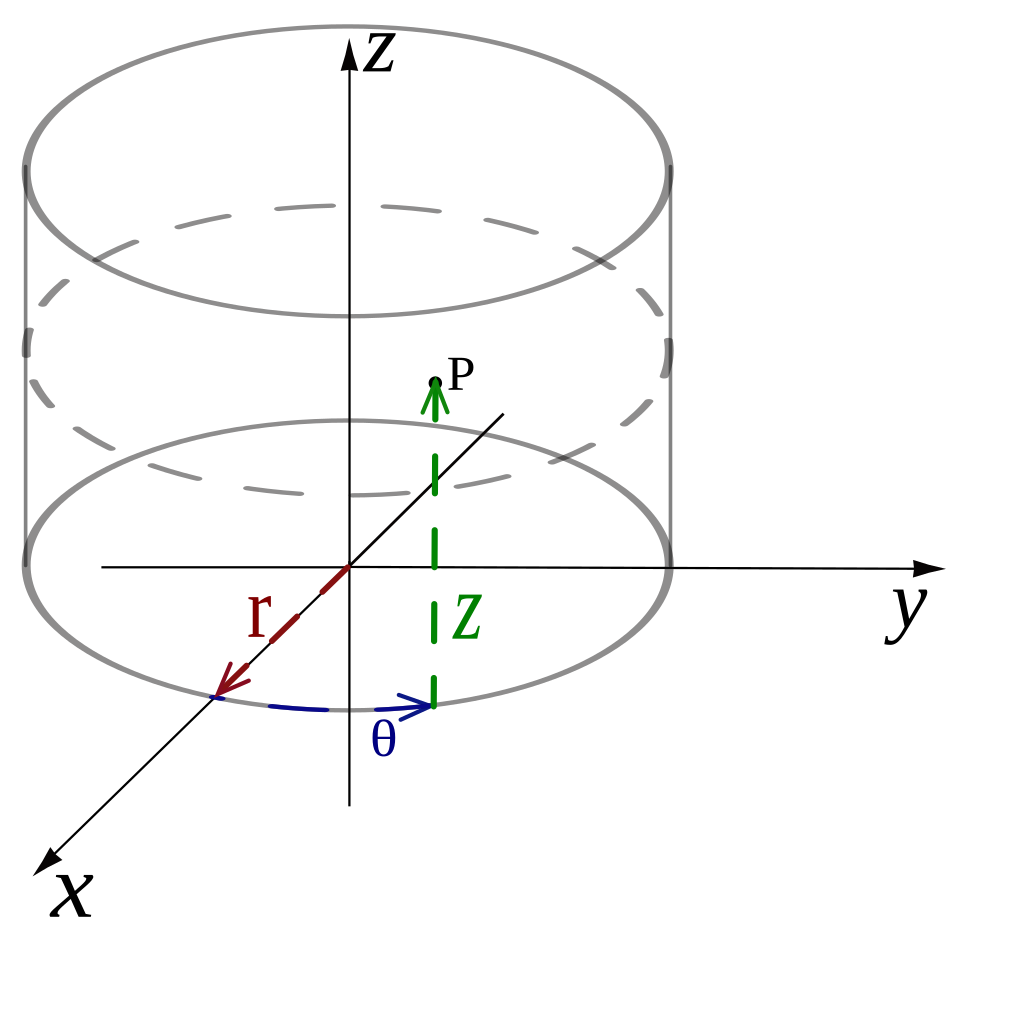
\includegraphics[width=8cm]{Fig/Cylindrical_coordinates2.svg.png}
\caption{Sylindriske koordinater. Kilde: \href{https://no.wikipedia.org/wiki/Polarkoordinatsystem}{Wikipedia},  \href{https://creativecommons.org/licenses/by-sa/3.0/}{CC-BY-SA}}\end{center}
\end{figure}
\begin{oppsum}{Fra kartesisk til sylindrisk}
Vi la $x,y,z$ være de vanlige kartesiske koordinater. For sylinderkoordinater $(r,\theta,z)$ har vi
\[
x = r \cos \theta, \quad y = r \sin \theta, \quad z = z
\]
\end{oppsum}
For et integral i sylindriske koordinater trenger vi å vite hva volumelementet $dV$ blir i disse koordinatene. Hvis man beregner Jacobi determinant for disse koordinater og setter inn i \eqref{eq:volum_variablebytte} får man:

\begin{defn}{Volumelement i sylindriske coordinater}
\[
dV = r\, dz\, dr\, d\theta
\]
\end{defn}
\begin{figure}[ht]\centering
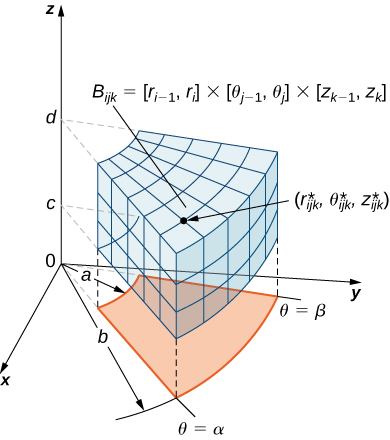
\includegraphics[width=8cm]{Fig/cylindrical_mesh.png}
\caption{Oppdeling av volumet i sylindriske koordinater, Kilde: \cite{SaH}, \href{https://creativecommons.org/licenses/by-nc-sa/4.0/}{CC BY-NC-SA 4.0}.}
\end{figure}
Området $E$ vi integrerer over blir omskrevet slik:
\begin{align*}
E &= \{(x, y, z) \mid (x, y) \in D,\, u_1(x, y) \leq z \leq u_2(x, y)\} \\
&= \{(r, \theta, z) \mid \alpha \leq \theta \leq \beta,\, h_1(\theta) \leq r \leq h_2(\theta),\, u_1(r \cos\theta, r \sin\theta) \leq z \leq u_2(r \cos\theta, r \sin\theta)\}
\end{align*}
Et trippelintegral i sylindriske koordinater er dermed:
\[
\iiint_E f(x, y, z)\, dV = \int_{\alpha}^{\beta} \int_{h_1(\theta)}^{h_2(\theta)} \int_{u_1(r \cos\theta, r \sin\theta)}^{u_2(r \cos\theta, r \sin\theta)} r\, f(r \cos\theta, r \sin\theta, z)\, dz\, dr\, d\theta
\]
\begin{rem}{Vær obs ved konvertering!}
Ikke glem å inkludere faktoren $r$, og sørg for å konvertere alle $x$- og $y$-variabler til sylindriske koordinater.
\end{rem}
\begin{eks}{}
Evaluer:

\[
\iiint_E y\, dV
\]
der $E$ er området som ligger under planet $z = x + 2$, over $xy$-planet, og mellom sylindrene $x^2 + y^2 = 1$ og $x^2 + y^2 = 4$.
\end{eks}
\begin{eks}{}
Konverter følgende integral til sylindriske koordinater:
\[
\int_{-1}^1 \int_0^{\sqrt{1 - y^2}} \int_{\sqrt{x^2 + y^2}}^{x^2 + y^2} xyz\, dz\, dx\, dy
\]
\end{eks}

\subsection{Trippelintegraler i kulekoordinater}

Et annet koordinatsystem som dukker opp ofte i anvendelser er kulekoordinater. I det tredimensjonale rommet $\mathbb{R}^3$ angir vi i kulekoordinater et punkt $P$ ved hjelp av avstanden $\rho$ fra origo,
polvinkelen $\theta$ fra den positive $x$-aksen (samme som i det
sylindriske koordinatsystemet), og vinkelen $\varphi$ fra den positive
$z$-aksen og linjen $\textbf{0}P$ (se \Cref{fig:kule}). Merk at $\rho > 0$ og
$0 \leq \varphi \leq \pi$ (ikke $2\pi$!). Kulekoordinater er nyttige for trippelintegraler over områder som er symmetriske med hensyn til origo.

\begin{figure}[ht]\begin{center}
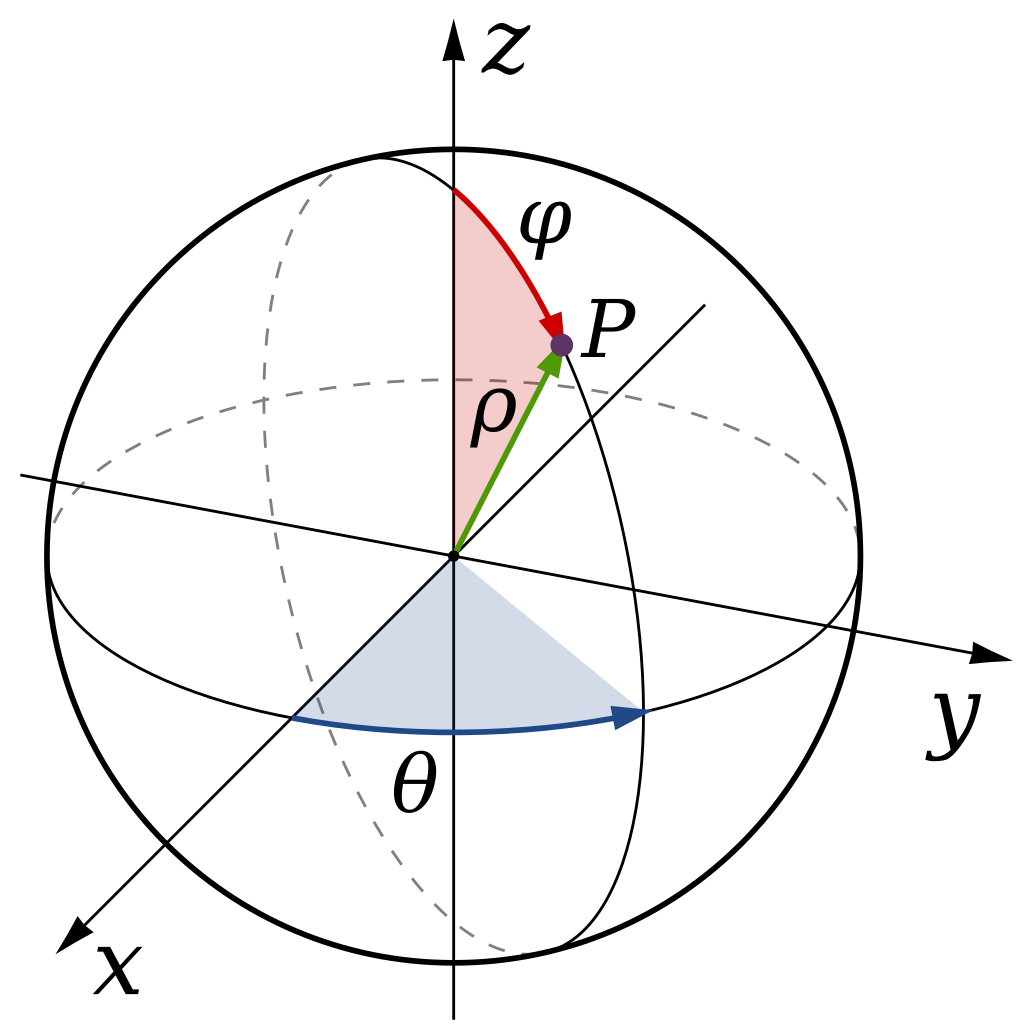
\includegraphics[width=8cm]{Fig/Spherical_Coordinates_(Colatitude,_Longitude).svg.png}
\caption{Kulekoordinater, Kilde \href{https://no.wikipedia.org/wiki/Polarkoordinatsystem}{Wikipedia}, open domain. }\end{center} \label{fig:kule}
\end{figure}

\begin{oppsum}{Konverteringsformlene til kulekoordinater}
Kulekoordinater $(\rho, \varphi, \theta)$ er relatert til kartesiske koordinater $(x,y,z)$ som:
\begin{align*}
x = \rho \sin \varphi \cos \theta, \quad y = \rho \sin \varphi \sin \theta, \quad z = \rho \cos \varphi \\
\text{ slik at: }
\rho \geq 0, \quad 0 \leq \varphi \leq \pi, \quad \text{ og } 0 \leq  \theta \leq 2\pi
\end{align*}
Omvendt, fra rektangulære koordinater til kulekoordinater kan vi bruke:
\[
\rho^{2} = x^{2} + y^{2} + z^{2}, \qquad 
\tan \theta = \frac{y}{x}, \qquad 
\varphi = \arccos\!\left(\frac{z}{\sqrt{x^{2} + y^{2} + z^{2}}}\right).
\]
\end{oppsum}
Se \Cref{sect:koordinater} for mer konverteringsformler.
\begin{rem}{To konvensjoner}
Det finnes to navnkonvensjoner for kulekoordinater. Vi bruker den matematiske konvensjonen. I fysikken (og noen praktiske anvendelser) er konvensjonen å bytte $\theta$ og $\varphi$. I tillegg skriver de gjerne $r$ i stedet for $\rho$ for avstand. Vi tar her $\rho$ for å skille det fra avstand til origo som er i bruk i sylinder- og polarkoordinater.

Vær forsiktig hvilken konvensjon en kilde bruker! 
\end{rem}
I likhet med polar- og sylinderkoordinater endrer volumelementet seg når vi bytter til kulekoordinater i integrasjonen. Det nye elementet kan enten utledes ved hjelp av geometriske betraktninger (se \Cref{fig:volum_kulekoord}) eller ved hjelp av variabelbytteformelen for trippelintegraler.


\begin{figure}[ht]\centering
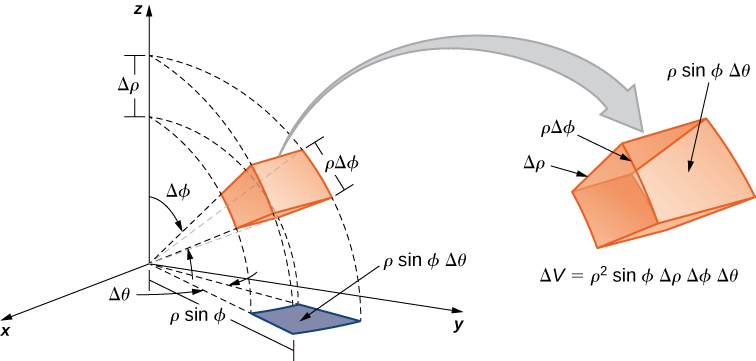
\includegraphics[width=10cm]{Fig/sperical_int.png}
\caption{Volumelement i kulekoordinater, Kilde: \cite{SaH}, \href{https://creativecommons.org/licenses/by-nc-sa/4.0/}{CC BY-NC-SA 4.0}.}\label{fig:volum_kulekoord}
\end{figure}
\begin{defn}{Volumelement i kulekoordinater}
\[
dV = \rho^2 \sin \varphi \, d\rho \, d\theta \, d\varphi
\]
\label{defn:volum_sfærisk}
\end{defn}
Vi begrenser området $E$ til en sfærisk kile med variabelgrenser:
\[
a \leq \rho \leq b, \quad \alpha \leq \theta \leq \beta, \quad \delta \leq \varphi \leq \gamma
\]
Et trippelintegral i kulekoordinater skrives da som:
\[
\iiint_E f(x, y, z)\, dV = \int_{\delta}^{\gamma} \int_{\alpha}^{\beta} \int_a^b \rho^2 \sin \varphi \, f(\rho \sin \varphi \cos \theta, \rho \sin \varphi \sin \theta, \rho \cos \varphi)\, d\rho \, d\theta \, d\varphi
\]
Det ser ikke bra ut men siden integralgrensene er konstant er det i praksis relativt lett å beregnes.
\begin{eks}{}
Beregn
\[
\iiint_E 8z\, dV, \quad \text{der } E \text{ er øvre halvkule: } x^2 + y^2 + z^2 = 1, z\geq 0
\]
Grensene er:
\[
0 \leq \rho \leq 1, \quad 0 \leq \theta \leq 2\pi, \quad 0 \leq \varphi \leq \frac{\pi}{2}
\]
og dermed 
\begin{align*}\iiint_E 8z dV &=  \int_0^{\pi/2}\int_0^{2\pi} \int_0^1 8\rho^3 \sin \varphi \cos \varphi \,d\rho\, d \theta \, d\varphi = \pi \int_{0}^{\pi/2}  \sin(2\varphi)\, d\varphi \\
&= -\pi \cos{2\varphi}|_0^{\pi/2}=2\pi \end{align*}
\end{eks}

\begin{eks}{}
Evaluer:
\[
\iiint_E zx\, dV
\]
der $E$ ligger innenfor kulen $x^2 + y^2 + z^2 = 4$ og under kjeglen med vinkel $\varphi = \frac{2\pi}{3}$ og betingelsen $x \leq 0$.
Grensene er:
\[
0 \leq \rho \leq 2, \quad \frac{2\pi}{3} \leq \varphi \leq \pi, \quad \frac{\pi}{2} \leq \theta \leq \frac{3\pi}{2}
\]
\end{eks}
\begin{eks}{}
Konverter følgende integral til kulekoordinater:
\[
\int_0^3 \int_0^{\sqrt{9 - y^2}} \int_{\sqrt{x^2 + y^2}}^{\sqrt{18 - x^2 - y^2}} x^2 + y^2 + z^2 \, dz \, dx \, dy
\]
Dette tilsvarer et område i første oktant, med:
\[
0 \leq \rho \leq 3\sqrt{2}, \quad 0 \leq \theta \leq \frac{\pi}{2}, \quad 0 \leq \varphi \leq \frac{\pi}{4}
\]
Integralet blir:
\[
\int_0^{\pi/4} \int_0^{\pi/2} \int_0^{3\sqrt{2}} \rho^4 \sin \varphi \, d\rho \, d\theta \, d\varphi
\]
\end{eks}

\begin{eks}{Snitt av en kegle og kule I}
La $E$ være området som er begrenset nedenfra av kjeglen 
$z = \sqrt{x^{2} + y^{2}}$
og ovenfra av kulen $x^{2} + y^{2} + z^{2} = 1$
(se \Cref{fig:cone_sphere}). Bruk konverteringsformlene til å skrive ligningene for kulen og kjeglen i kulekoordinater. For kulen:
\[
x^{2} + y^{2} + z^{2} = 1 
\quad \Rightarrow \quad 
\rho^{2} = 1 
\quad \Rightarrow \quad 
\rho = 1.
\]
For kjeglen:
\[
z = \sqrt{x^{2} + y^{2}}
\quad \Rightarrow \quad 
\rho \cos \varphi = \rho \sin \varphi
\quad \Rightarrow \quad 
\tan \varphi = 1
\quad \Rightarrow \quad 
\varphi = \frac{\pi}{4}.
\]
Dermed blir integralet for volumet av området $E$:
\[
V(E) = \int_{0}^{2\pi} \int_{0}^{\pi/4} \int_{0}^{1} 
\rho^{2} \sin \varphi \, d\rho \, d\varphi \, d\theta = \frac{2\pi}{3}\left(1-\frac{\sqrt{2}}{2}\right).
\]
\end{eks}

\begin{figure} \centering
\usetikzlibrary{shadings,intersections}
\begin{tikzpicture}
  \coordinate (O) at (0,0);

  % ball background color
  \shade[ball color = blue, opacity = 0.2] (0,0) circle [radius = 2cm];
  % cone
  \begin{scope}
    \def\rx{0.71}% horizontal radius of the ellipse
    \def\ry{0.15}% vertical radius of the ellipse
    \def\z{0.725}% distance from center of ellipse to origin
    \path [name path = ellipse]    (0,\z) ellipse ({\rx} and {\ry});
    \path [name path = horizontal] (-\rx,\z-\ry*\ry/\z)
                                -- (\rx,\z-\ry*\ry/\z);
    \path [name intersections = {of = ellipse and horizontal}];

    % radius to base of cone in ball
    \draw[fill = gray!50, gray!50] (intersection-1) -- (0,0)
      -- (intersection-2) -- cycle;
    % base of cone in ball
    \draw[fill = gray!30, densely dashed] (0,\z) ellipse ({\rx} and {\ry});
  \end{scope}
  % label of cone
  \draw (0.25,0.4) -- (0.9,0.1) node at (1.05,0.0) {kegle};

  % ball
  \draw (O) circle [radius=2cm];
  % label of ball center point
  \filldraw (O) circle (1pt) node[below] {origo};
  % radius
  \draw[] (O) to [] (-1.33,1.33);
  \draw[] (O) -- (1.33,1.33);

  % cut of ball surface
  \draw[red] (-1.35,1.47) arc [start angle = 140, end angle = 40,
    x radius = 17.6mm, y radius = 14.75mm];
  \draw[red, densely dashed] (-1.36,1.46) arc [start angle = 170, end angle = 10,
    x radius = 13.8mm, y radius = 3.6mm];
  \draw[red] (-1.29,1.52) arc [start angle=-200, end angle = 20,
    x radius = 13.75mm, y radius = 3.15mm];

  % label of cut of ball surface
  \draw (-1.2,2.2) -- (-0.53,1.83) node at (-1.37,2.37) {volum};
\end{tikzpicture}
\caption{Snitt av en kule og en kegle, fra \href{https://texample.net/steradian-cone-sphere/}{Bartman}, \href{https://creativecommons.org/licenses/by-sa/4.0/}{CC BY-SA 4.0}}
\label{fig:cone_sphere}
\end{figure}

Siden integrasjonsgrensene ikke er avhengige av variablene, kan vi i siste eksempel også lett bytte integrasjonsrekkefølge. Situasjonen er vanskeligere hvis vi har integralgrenser som er avhengige av hverandre.

\begin{eks}{Snitt av en kegle og kule II}
La $M$ være området som er begrenset nedenfra av kjeglen 
$z = \sqrt{x^{2} + y^{2}}$
og ovenfra av kulen $x^{2} + y^{2} + z^{2} = z$. Sett opp et trippelintegral i kulekoordinater og finn volumet av området ved å bruke følgende integrasjonsrekkefølger:
\begin{align*}
a)\quad d\rho \, d\varphi \, d\theta \qquad b)\quad d\varphi \, d\rho \, d\theta
\end{align*}
a) Dermed er for kulen:
\[
x^{2} + y^{2} + z^{2} = z
\quad \Rightarrow \quad 
\rho^{2} = \rho \cos (\varphi) 
\quad \Rightarrow \quad 
\rho = \cos (\varphi).
\]
For kjeglen:
\[
z = \sqrt{x^{2} + y^{2}}
\quad \Rightarrow \quad 
\rho \cos \varphi = \rho \sin \varphi
\quad \Rightarrow \quad 
\tan \varphi = 1
\quad \Rightarrow \quad 
\varphi = \frac{\pi}{4}.
\]
Dermed blir integralet for volumet av området $E$:
\[
V(E) = \int_{0}^{2\pi} \int_{0}^{\pi/4} \int_{0}^{\cos (\varphi)} 
\rho^{2} \sin \varphi \, d\rho \, d\varphi \, d\theta.
\]
b) Betrakt $\varphi\rho$-planet. Merk at områdene for $\varphi$ og $\rho$ (fra del a) er
\[
0 \leq \varphi \leq \frac{\pi}{4}, 
\qquad 0 \leq \rho \leq \cos (\varphi).
\]
Kurven $\rho = \cos \varphi$ skjærer linjen $\varphi = \pi/4$ i punktet $\left(\tfrac{\pi}{4}, \tfrac{\sqrt{2}}{2}\right)$.
For å endre integrasjonsrekkefølgen må vi derfor bruke to delområder:
\[
0 \leq \rho \leq \tfrac{\sqrt{2}}{2}, 
\qquad 0 \leq \varphi \leq \tfrac{\pi}{4},
\]
og
\[
\tfrac{\sqrt{2}}{2} \leq \rho \leq 1, 
\qquad 0 \leq \varphi \leq \arccos \rho.
\]
Dermed blir integralet for volumet av området $E$:
\[
V(E) = \int_{0}^{2\pi} 
\int_{0}^{\tfrac{\sqrt{2}}{2}} 
\int_{0}^{\pi/4} 
\rho^{2} \sin \varphi \, d\varphi \, d\rho \, d\theta
+ \int_{0}^{2\pi} 
\int_{\tfrac{\sqrt{2}}{2}}^{1} 
\int_{0}^{\arccos \rho} 
\rho^{2} \sin \varphi \, d\varphi \, d\rho \, d\theta.
\]
I begge tilfeller blir resultatet av integrasjonen
\[
V(E) = \frac{\pi}{8}.
\]
\end{eks}

\subsection{Anvendelse: Treghetsmoment }
Den kinetiske energien til en partikkel med masse \( m \) og hastighet \( v \) er
\[
\text{KE} = \frac{1}{2}mv^2.
\]
Massens størrelse uttrykker dens treghet, som er dobbelt så stor som energien den har når hastigheten er én enhet.

Hvis partikkelen beveger seg i en sirkel med radius \( D \), er vinkelhastigheten \( \Omega \) (i radianer per tidsenhet), og den translasjonelle hastigheten er
\[
v = \Omega D.
\]
Anta at et stivt legeme roterer med vinkelhastighet \( \Omega \) rundt en akse \( L \). Dersom legemet på et tidspunkt fyller en region \( R \), og har tetthet \( \delta = \delta(x, y, z) \), så har hvert masseelement \( dm = \delta\, dV \) kinetisk energi
\[
d\text{KE} = \frac{1}{2} v^2 dm = \frac{1}{2} \delta \Omega^2 D^2\, dV,
\]
der \( D = D(x, y, z) \) er avstanden til rotasjonsaksen \( L \). Den totale kinetiske energien til det roterende legemet er derfor
\[
\text{KE} = \frac{1}{2} \Omega^2 \iiint_R D^2 \delta\, dV = \frac{1}{2} I \Omega^2,
\text{ hvor } I = \iiint_R D^2 \delta\, dV
\]
kalles \emph{treghetsmomentet} om aksen \( L \).

Treghetsmomentet spiller samme rolle i uttrykket for rotasjonsenergi (i form av vinkelhastighet) som massen gjør i uttrykket for translasjonsenergi (i form av lineær hastighet). Når \( \Omega = 1 \), er treghetsmomentet dobbelt så stort som den kinetiske energien.

Vi definerer \emph{treghetsradiusen} \( D \) som den verdien av \( D_0 \) som gir lik kinetisk energi:
\[
m D^2 = I \quad \Rightarrow \quad D = \left( \frac{1}{m} \iiint_R D^2 \delta\, dV \right)^{1/2},
\text{ der } m = \iiint_R \delta\, dV.
\]

\begin{eks}{}
Treghetsmomentet om \( z \)-aksen til et legeme med tetthet \( \delta \), som fyller regionen \( R \), er gitt ved integralet
\[
I = \iiint_R (x^2 + y^2)\, \delta\, dV.
\]
Beregn dette treghetsmomentet for et legeme med $\delta\equiv 1$ som fyller området inne i kulen \( x^2 + y^2 + z^2 = 4a^2 \) og utenfor sylinderen \( x^2 + y^2 = a^2 \).
I kulekoordinater er treghetsmomentet gitt som
\[
I = 2\int_0^{2\pi}d \theta \int_{\pi/6}^{\pi /2} \sin \phi d \phi \int_{a/\sin \phi}^{2a} \rho^42 \sin^2\phi \rho^2\, d\rho.
\]
I sylindriske koordinater er det
\[
I = 2\int_0^{2\pi} d\theta \ \int_a^{2a} r\, dr \int_0^{\sqrt{4a^2 - r^2}} r^2\, dz.
\]
Det siste uttrykket ser enklere ut. Vi fortsetter med det. Evaluer \( \theta \)- og \( z \)-integralene, for å få
\[
I = 4\pi \int_a^{2a} r^3 \sqrt{4a^2-r^2}\, dr.
\]
Ved substitusjonen \( u = 4a^2 - r^2 \), \( du = -2r\, dr \), får vi
\[
I = 2\pi \int_{0}^{3a^2} (4a^2 - u)\sqrt{u}\, du = 2\pi \left| 4a^2 \frac{u^{3/2}}{3/2} - \frac{u^{5/2}}{5/2} \right|_{0}^{3a^2} du = \frac{44}{5}\sqrt{3}\pi a^5
\]
\end{eks}

\section{Numerisk beregning av trippelintegraler}\label{sect:num_met1}
For å lage en numerisk integrasjonsregel for trippelintegraler må vi forstå hvordan trippelintegraler egentlig er definert. Anta at vi skal integrere over en boks. Vi kan definere en rektangulær boks \( B \subset \mathbb{R}^3 \) som
\[
B = \{ (x, y, z) \mid a \leq x \leq b,\, c \leq y \leq d,\, e \leq z \leq f \}.
\]
\begin{figure}[ht] \centering
\tdplotsetmaincoords{70}{120} % view angle
\begin{tikzpicture}[tdplot_main_coords, scale=1.2]
  % Draw large box 
  \draw[thick, cyan, fill=cyan!10, opacity=0.5] (0,0,0) -- (4,0,0) -- (4,3,0) -- (0,3,0) -- cycle; % bottom
  \draw[thick, cyan, fill=cyan!10, opacity=0.5] (0,0,2) -- (4,0,2) -- (4,3,2) -- (0,3,2) -- cycle; % top
  \draw[thick, cyan, opacity=0.5] (0,0,0) -- (0,0,2);
  \draw[thick, cyan, opacity=0.5] (4,0,0) -- (4,0,2);
  \draw[thick, cyan, opacity=0.5] (4,3,0) -- (4,3,2);
  \draw[thick, cyan, opacity=0.5] (0,3,0) -- (0,3,2);

  % Draw axes
  \draw[->] (4.5,0,0) --++ (1,0,0) node[anchor=north east] {$x$};
  \draw[->] (4.5,0,0) --++ (0,1,0) node[anchor=north west] {$y$};
  \draw[->] (4.5,0,0) --++ (0,0,1) node[anchor=south] {$z$};

  % Draw small box inside
  \coordinate (Bcenter) at (1,.5,.25);
  \def\dx{0.5}
  \def\dy{0.5}
  \def\dz{0.5}
  \path (Bcenter) ++(-\dx/2,-\dy/2,-\dz/2) coordinate (A);
  \draw[thick, orange, fill=orange!30, opacity=0.6] (A) ++(0,0,0) coordinate (O)
    --++ (\dx,0,0) coordinate (X) 
    --++ (0,\dy,0) coordinate (XY)
    --++ (-\dx,0,0) coordinate (Y)
    -- cycle; % bottom

  \draw[thick, orange, fill=orange!30, opacity=0.6] (O) --++ (0,0,\dz) coordinate (OZ)
    --++ (\dx,0,0) coordinate (XZ)
    --++ (0,\dy,0) coordinate (XYZ)
    --++ (-\dx,0,0) coordinate (YZ)
    --++ (0,-\dy,0); % top

  \draw[thick, orange, opacity=0.6] (O) -- (OZ);
  \draw[thick, orange, opacity=0.6] (X) -- (XZ);
  \draw[thick, orange, opacity=0.6] (XY) -- (XYZ);
  \draw[thick, orange, opacity=0.6] (Y) -- (YZ);

  % Zoom line
  \draw[thick, ->] (Bcenter) ++(1,1.1,0.5) --++ (1,5.5,2);

  % Enlarged version
  \begin{scope}[shift={(1,7,2)}, scale=1.5]
    \draw[thick, orange, fill=orange!30, opacity=0.6] (0,0,0) --++ (\dx,0,0) --++ (0,\dy,0) --++ (-\dx,0,0);
    \draw[thick, orange, fill=orange!30, opacity=0.6] (0,0,0) --++ (0,0,\dz) --++ (\dx,0,0) --++ (0,0,-\dz);
    \draw[thick, orange, fill=orange!30, opacity=0.6] (0,0,0) --++ (0,\dy,0) --++ (0,0,\dz) --++ (0,-\dy,0) ;
    \draw[thick, orange, opacity=0.6] (0,\dy,0) --++ (0,0,\dz);
    \draw[thick, orange, opacity=0.6] (\dx,\dy,0) --++ (0,0,\dz);
    \draw[thick, orange, opacity=0.6] (\dx,0,0) --++ (0,0,\dz);
    \draw[thick, orange, opacity=0.6] (0,0,\dz) --++ (\dx,0,0) --++ (0,\dy,0) --++ (-\dx,0,0);

    % Axes and dimensions
    \draw[<->] (\dx/4,.75,0) --++ (\dx,0,0) node[midway, below] {\quad $\Delta x$};
    \draw[<->] (.75,-\dy/8,0) --++ (0,\dy,0) node[midway, below] {$\Delta y$};
    \draw[<->] (0.5,1,\dz/2) --++ (0,0,\dz) node[midway, right] {$\Delta z$};
  \end{scope}

  % Label box B
  \node at (2,8,3.5) {$B_{ijk}$};

\end{tikzpicture}
\caption{Oppdeling av en boks i små bokser}\label{3Dbox}
\end{figure}
Vi deler intervallet \( [a, b] \) inn i \( l \) delintervaller \( [x_{i-1}, x_i] \), intervallet \( [c, d] \) inn i \( m \) delintervaller \( [y_{j-1}, y_j] \) og \( [e, f] \) inn i \( n \) delintervaller \( [z_{k-1}, z_k] \) av lik lengde:
\[
\Delta x = \frac{x_i - x_{i-1}}{l}, \qquad \Delta y = \frac{y_j - y_{j-1}}{m}, \qquad \Delta z = \frac{z_k - z_{k-1}}{n}.
\]
Da er den rektangulære boksen \( B \) delt inn i \( lmn \) delbokser  (se \Cref{3Dbox}):
\[
B_{ijk} = [x_{i-1}, x_i] \times [y_{j-1}, y_j] \times [z_{k-1}, z_k].
\]
Da er trippelintegralet definert som grenseverdien av Riemann-summen
\[
\sum_{i=1}^{l} \sum_{j=1}^{m} \sum_{k=1}^{n} f(x^{*}_{ijk}, y^{*}_{ijk}, z^{*}_{ijk}) \, \Delta x \, \Delta y \, \Delta z.
\]
Dermed kan vi lage numeriske tilnærminger som i 2D ved å kutte opp den store boksen inn i småbiter og summere verdier til funksjonen som skal integreres.
I Python betyr det at vi lager gitter ved hjelp av numpy og evaluerer funksjoner på gitteren for å lage disse approksimasjoner.

\begin{oppsum}{Numpy og Scipy kommandoer for multiintegraler}

\begin{minipage}{.9\columnwidth}
\begin{lst}{}
import numpy as np

import scipy as sp

np.meshgrid

sp.integrate.tplquad
\end{lst}
\end{minipage}
\textbf{OBS:} meshgrid kan lage flerdimensjonale gitter og det er avhengig av antall variabler den får hva slags gitter den lager.
\end{oppsum}
Sjekk JuPyter notater om integrasjon av funksjoner og diskrete verdier.

Vi ser på gittermetoden som en forberedelse for de numeriske metoder for partielle differensiallikninger vi skal studere i del 3 av notatene.
\newpage
\section{Linjeintegraler}\label{sect:linint1}

I dette delkapitlet introduserer vi en ny type integral: Nemlig linjeintegralet, hvor vi ønsker å integrere en funksjon langs en gitt kurve. Det viser seg at det er forskjellige måter å definere disse integralene på, avhengig av hva man ønsker å beregne. Først skal vi se på linjeintegral av funksjoner. Senere skal vi se på linjeintegral av vektorfelter.

%\subsection{linjeintegral av funksjoner}
Vi antar at leseren er kjent med grunnleggende egenskaper ved kurver fra tidligere kurs. La oss minne om
\begin{defn}{Parametriseringer og tangenter}
En kurve $C$ er en delmengde av $\R^n$ som kan beskrives som bildet av en deriverbar funksjon $\vect{r}\colon [a,b] \rightarrow \R^n$. Man kaller $\vect{r}$ en \emph{parametrisering} av $C$.

Hver parametrisering definerer en \emph{tangentvektor} til kurven \[\vect{r}'(t):=\lim_{h\rightarrow 0}\frac{\vect{r}(t+h)-\vect{r}(t)}{h}, \qquad t \in [a,b].\]\label{defn:para_tangent}
\end{defn}
Vi viser noen vanlige parametriseringer for enkelte vanlige funksjoner i \Cref{table:para}. 

Merk at mengden $C$ tillater mange forskjellige parametriseringer. For eksempel kan sirkelen $C=\{(x,y) \colon x^2+y^2 = r^2\}$ parametriseres som gitt i \Cref{table:para}, men vi kan også velge en parametrisering som løper gjennom sirkelen med dobbel hastighet:
\begin{align}\label{para:doublespeed}
x= r\cos (2t), \quad y= r \sin (2t), \quad 0 \leq t \leq \pi
\end{align}
Vi kan altså bruke mange forskjellige parametriseringer av en kurve $C$ i $\R^n$. La oss nå se på en vilkårlig parameterisering
\[\vect{r}(t)=(r_1(t),..., r_n(t))^\top.\]
Tangentvektoren blir da
\begin{align}\label{tangentvect}\vect{r}^\prime(t):=\frac{d\vect{r}}{dt}(t)=\left(\frac{dr_1}{dt}(t),...,\frac{dr_n}{dt}(t)\right)^\top,\end{align}
med lengde \(\|\vect{r}^\prime\|=\sqrt{\frac{d\vect{r}}{dt}\cdot\frac{d\vect{r}}{dt}}=\sqrt{\left(\frac{dr_1}{dt}\right)^2+...+\left(\frac{dr_n}{dt}\right)^2}.\)
For en slik parametrisering har vi at et buelengde-element $ds$ for en kurve $\mathcal{C}$ i $\R^n$ er gitt som 
\[ds=\sqrt{dr_1^2+...dr_n^2}.\]
Med dette begrepsapparatet kan vi nå definere linjeintegralet på følgende vis.

\begin{figure}[ht]\centering
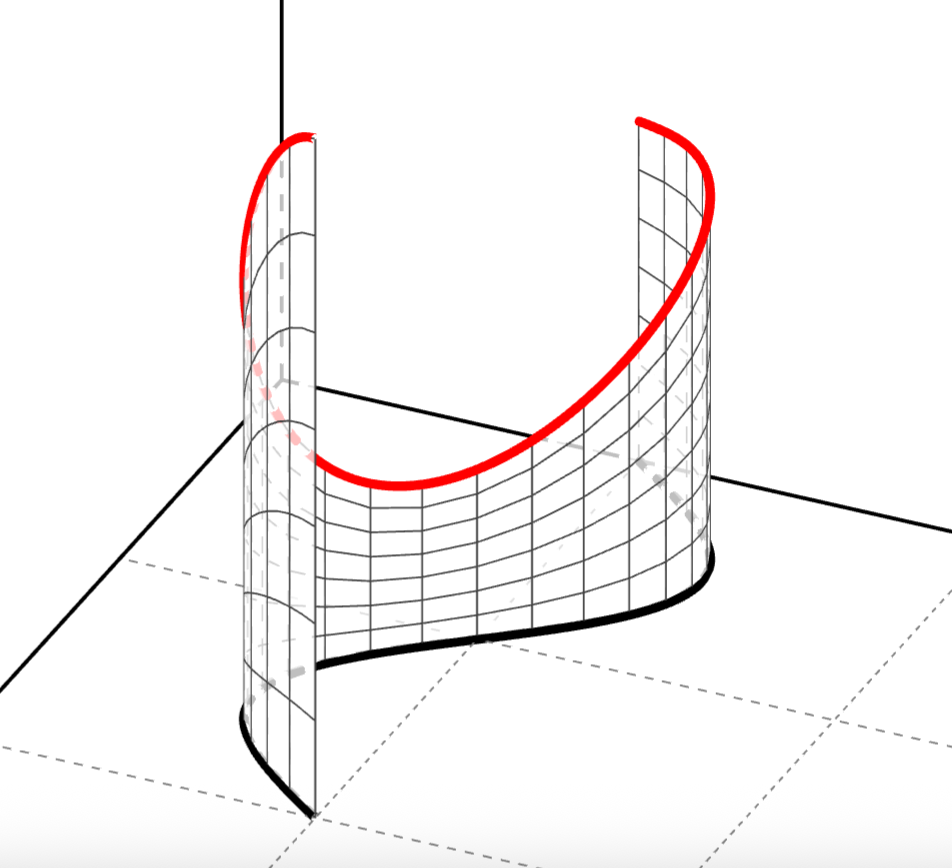
\includegraphics[width=7cm]{Fig/kurve_func.png}
\caption{En 2D kurve $\mathcal{C}$ (svart linje i xy-planet) sammen med funksjonsverdier til en funksjon $f$ (rødt). \href{https://www.geogebra.org/m/us62espz}{interaktiv Geogebra versjon} Merk: Parametriseringen av $\mathcal{C}$ er ikke synlig i figuren.}
\end{figure}

\begin{defn}{Linjeintegral av funksjon på parameterkurve}
Gitt \( f\colon \R^n \rightarrow \R \) og en kurve $\mathcal{C}$ med parametrisering \(\vect{r} \colon [a,b] \rightarrow \R^n, \vect{r}(t)=(r_1(t),\ldots, r_n(t))^\top\), så er \emph{linjeintegralet} langs $\mathcal{C}$ (eller langs \( \vect{r}(t) \)) definert som:
\[
\int_\mathcal{C} f\, ds = \int_a^b f(\vect{r}(t))\, \|\vect{r}'(t)\|\, dt,
\]
hvor \(\|\vect{r}'(t)\| \) er definert som i \eqref{tangentvect}.
\end{defn}
Dersom funksjonen vi integrerer er $f=1$ så får vi naturligvis buelengden til kurven.
\begin{defn}{Buelengde}
Hvis $\mathcal{C}$ er en glatt kurve med parametrisering $\vect{r} \colon [a,b]\rightarrow \R^n$ så er
\[\text{buelengden til }\mathcal{C} \quad L(\mathcal{C}):= L(\vect{r}) = \int_\mathcal{C} 1 ds = \int_a^b \lVert \vect{r}'(t)\rVert dt \]
\end{defn}

\begin{rem}{}
En bør merke seg at buelengde er definert positivt. Det vil si at $ds>0.$ Derfor er alltid $a<b$ i definisjonen av linjeintegralet for funksjoner.
\end{rem}
I denne sammenheng er det viktig å si et par ord om \textit{orientering.}
La oss anta at kurven \( \mathcal{C} \) er gitt ved parameteriseringen $\vect{r}(t)$, og at startpunktet på kurven er \( P \), og sluttpunktet er \( Q \).
Parameteriseringen \( \vect{r} \) bestemmer da en positiv \emph{orientering} av kurven, nemlig den retningen som kurven spores ut i når \( t \) øker.
La oss definere negativ, eller omvendt orientering.
\begin{defn}{Omvendt orientering}
\label{omvendt_orient}
For en kurve $\mathcal{C}$ lar vi \( -\mathcal{C} \) være kurven med de samme punktene som \( \mathcal{C} \), men hvor kurven starter i \( Q \) og slutter i \( P \), \textit{igjen med} \( t \) \textit{som øker mens vi følger kurven} (viktig!). Med andre ord: gitt en kurve \( \mathcal{C} \), er \( -\mathcal{C} \) den samme geometriske kurven som \( \mathcal{C} \), men med motsatt orientering. 
\end{defn}
Hvis vi bytter retningen til en kurve, endres ikke verdien av linjeintegralet, dvs.
\[ \int_\mathcal{C} f\, ds = \int_{-\mathcal{C}} f\, ds.\]
\begin{rem}{}
Dette noe uventede resultatet skyldes altså definisjonen av linjeintegralet over buelengde $s$. Som nevnt så er $ds$ alltid positiv, så øvre integrasjonsgrense er \textit{alltid} større enn nedre. Vi bør med andre ord merke oss at 
\[\int_\mathcal{C} f\, ds=\int_{-\mathcal{C}} f\, ds=\int_a^bf(\vect{r}(t))\|\vect{r}^\prime\|dt\]
En kan saktens lure på hva det da vil si å integrere fra $b$ til $a.$ Det naturlige vil være å definere dette som linjeintegralet av funksjonen $-f$. Vi får:
\[\int_\mathcal{C} -f\, ds=-\int_a^bf(\vect{r}(t))\|\vect{r}^\prime\|dt:=\int_b^af(\vect{r}(t))\|\vect{r}^\prime\|dt.\]
\end{rem}

\subsubsection{Notasjon i 2D og 3D}
For å holde diskusjonen konkret så kommer vi for det meste til å konsentrere oss om kurver i todimensjonale og tredimensjonale rom. Spesielt hvis vi bruker en parametrisering (f.eks. fra \Cref{table:para}), skriver vi kurven på formen \[\vect{r}(t) = (x(t),y(t))^\top\quad\textrm{(2D)}\] og \[\vect{r}(t) = (x(t),y(t),z(t))^\top\quad\textrm{(3D)}.\] Dette gir henholdsvis  
\[\lVert \vect{r}'(t)\rVert = \sqrt{(x'(t))^2+(y'(t))^2}\quad\text{(2D)}\qquad\textrm{og}\qquad\lVert \vect{r}'(t)\rVert = \sqrt{(x'(t))^2+(y'(t))^2+(z(t))^2}\quad\text{(3D)}.\]

\begin{eks}{}
La $C = \{(x,y) \colon x^2+y^2 = r^2\}$. Parametriser som i \Cref{table:para}:
\[\int_C 1 \mathrm{d}s =\int_0^{2\pi} 1\cdot \sqrt{r^2 (-\sin(t))^2 + (\cos (t))^2}dt = 2\pi r \]
Integralverdien er altså omkretsen av sirkelen! La oss nå regne med parametriseringen i \eqref{para:doublespeed}. Da får vi
\[\int_C 1\, d s = \int_0^{\pi} \sqrt{4r^2(\cos (2t)^2+\sin (2t)^2)}\, dt = \pi \cdot 2r = 2\pi r\]
Verdien er altså den samme som i forrige utregning. Mer generelt har vi at integralet er uavhengig av parametriseringen.
\end{eks}


\begin{eks}{}
Beregn $\int_{C_1} x^2+y\, ds$ der $C_1$ er linjen fra $(2,-1)$ til $(5,3)$ med parametrisering $\vect{r}(t)=((1-t)2+5t, (1-t)(-1)+3t))^\top=(2+3t,-1+4t)^\top$. Vi har $\lVert \vect{r}'(t)\rVert = 5$
\[\int_{C_1} x^2+4y\, ds = \int_0^1 ((2+3t)^2-4+16t)\cdot 5 dt =\int_0^1 (28t+9t^2)\cdot 5 dt = 85\]
La nå $C_2$ være den omvendte veien, dvs. linja fra $(5,3)$ til $(2,-1)$. Vi har en parametrisering $((1-t)5+t2,(1-t)3-t)^\top=(5-3t,3-4t)^\top$ som gir
\[\int_{C_2} x^2+4y\, ds = \int_0^1 ((5-3t)^2+12-16t)\cdot 5\, dt= \int_0^1 (37-46t+9t^2)\cdot 5\, dt= 85\]
\end{eks}

\begin{oppsum}{Regneregler for linjeintegraler}
  Vi kan regne med linjeintegraler som vanlig for integraler. Dette betyr at:
  \begin{align}
  \int_C (\lambda f+g)\, ds = \lambda \int_C f \, ds + \int_C g \, ds, \quad \lambda \in \R \label{lin_int_linear}\\
  \int_{C_1 \cup C_2} f \, ds = \int_{C_1} f \, ds + \int_{C_2} f \, ds \label{lin_int_add}
  \end{align}
  Her betyr notasjonen $C_1\cup C_2$ at kurven $C$ er sammensatt av to kurver. Spesielt kan vi dermed utvide definisjonen av integralet til stykkvis glatte kurver.
\end{oppsum}
\begin{rem}{Stykkevis glatte kurver}
Dersom en kurve er sammensatt av flere kurver \( C_1, C_2, \ldots, C_n \), da er:
\[
\int_C f(x, y)\, ds = \sum_{i=1}^n \int_{C_i} f(x, y)\, ds
\]
\end{rem}

\begin{eks}{En stykkvis glatt kurve sammensatt av tre deler}
Beregn \( \int_C 4x^3\, ds \), hvor \( C \) er en kurve bestående av tre segmenter:
\begin{itemize}
    \item \( C_1: x(t) = t,\, y(t) = -1,\quad -2 \leq t \leq 0 \)
    \item \( C_2: x(t) = t,\, y(t) = t^3 - 1,\quad 0 \leq t \leq 1 \)
    \item \( C_3: x(t) = 1,\, y(t) = t,\quad 0 \leq t \leq 2 \)
\end{itemize}
Summen av de tre integralene gir \( \int_C 4x^3\, ds = 9. \)
\end{eks}

\section{Parametriske flater og flateintegraler}\label{sect:flateint}

Vi skal nå se på hvordan man kan representere flater i 3D-rommet ved hjelp av parametrisering. På samme måte som en kurve i planet kan beskrives ved parametrene \( x = f(t),\ y = g(t) \), kan vi også beskrive flater i rommet ved å bruke to parametre. Merk at selv om ordet \textit{flate} høres veldig flatt ut, så er det ikke nødvendigvis det. En "flat" flate kaller vi for et \textit{plan.} Et eksempel på et plan er $xy$-planet. 
Ordet \textit{flate} er altså her brukt i vid forstand. For å guide intuisjonen kan du se for deg et øyeblikksbilde av et laken i vinden. Dette øyeblikksbildet er det intuitive bildet vi må ha når vi snakker om flater i matematikken. Kanskje ville "overflate" vært et bedre begrep enn "flate," men dessverre er det lite vi får gjort med inngrodd terminologi\footnote{En av oss insisterer på at \textit{laken} er ordet vi bør bruke i stedet for \textit{flate}. Men vi velger å beholde ordet \textit{flate}.}.


\begin{defn}{Parametrisk flate}
En \emph{parametrisk flate} i 3D er en kontinuerlig deriverbar vektorfunksjon av to variabler:
\[
\vect{r}(u, v) = x(u, v)\, \vect{i} + y(u, v)\, \vect{j} + z(u, v)\, \vect{k}
\]
hvor \( (u, v) \) tilhører et område \( D \subseteq \mathbb{R}^2 \).

Denne parameteriseringen spenner ut en flate i \( \mathbb{R}^3 \). For hvert punkt \( (u, v) \in D \) får vi et punkt \( (x(u,v), y(u,v), z(u,v)) \) på flaten.
\end{defn}
Utfordringen når det gjelder flater er å finne en god parametrisering. I det følgende kommer noen eksempler på typiske flater og parametriseringer.
\begin{eks}{Parametrisering av sylinder, omdreiningsflate og kule}
Når vi så på forskjellige koordinatsystemer i 3D var det noen objekter som gikk igjen. La oss parametrisere overflaten til noen av dem. 
\begin{itemize}
    \item En sylinder med radius $R$ og høyde $H$:
    \[
    \vect{r}(u,v) = R\cos u\, \vect{i} + R\sin u\, \vect{j} + v\, \vect{k}, \quad 0 \leq u \leq 2\pi,\ 0 \leq v \leq H
    \]
    \item En kule med radius \( a \):
    \[
    \vect{r}(u,v) = a \sin u \cos v\, \vect{i} + a \sin u \sin v\, \vect{j} + a \cos u\, \vect{k}, \quad 0 \leq u \leq \pi,\ 0 \leq v \leq 2\pi
    \]
\end{itemize}
\end{eks}

\begin{eks}{Parametrisering av trekanter}\mbox{}\label{ex:trekant_para}\\
\begin{minipage}{7cm}
En trekant $T$ med hjørner $\vect{u},\vect{v},\vect{w}$ kan parametriseres slik
\[\vect{r}(s,t):=\vect{u}+s(\vect{v}-\vect{u})+t(\vect{w}-\vect{u}),\]
hvor $ 0\leq s\leq 1, 0\leq t\leq 1-s$.

Tilsvarende kan man parametrisere konvekse geometriske figurer som ligger i et plan.
\end{minipage}
\begin{minipage}{7cm}
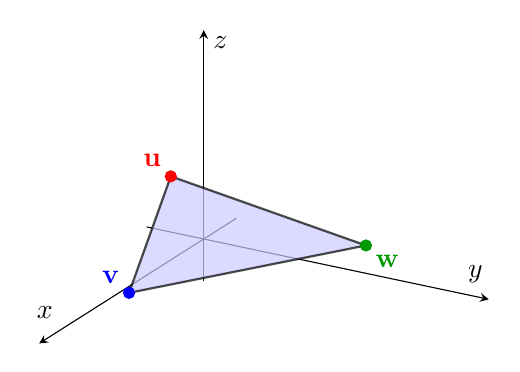
\begin{tikzpicture}
  \begin{axis}[
    view={120}{30},
    xlabel=$x$, ylabel=$y$, zlabel=$z$,
    axis lines=center,
    ticks=none,
    xmin=-1, xmax=5,
    ymin=-1, ymax=5,
    zmin=-1, zmax=5
  ]

  % Define the three vectors u, v, w
  \addplot3 [mark=*, color=red] coordinates {(1,0,2)} node[above left] {$\mathbf{u}$};
  \addplot3 [mark=*, color=blue] coordinates {(4,1,1)} node[above left] {$\mathbf{v}$};
  \addplot3 [mark=*, color=green!60!black] coordinates {(2,4,2)} node[below right] {$\mathbf{w}$};

  % Fill triangle between the three points
  \addplot3[
    fill=blue!20,
    draw=black,
    opacity=0.7,thick
  ]
  coordinates {
    (1,0,2)
    (4,1,1)
    (2,4,2)
    (1,0,2) % Close the triangle
  };
  \end{axis}
\end{tikzpicture}
\end{minipage}
\end{eks}

\subsection{Omdreiningsflater}
Et omdreiningslegeme er i geometrien et legeme som fremkommer ved at en plan figur dreier seg om en akse som ligger i samme plan som figuren. Overflaten av et omdreiningslegeme er derfor en omdreiningsflate.

Når vi skal studere omdreiningsflater så er det naturlig å benytte seg av sylinderkoordinater; $\vect{r}=(r\cos \varphi ,r \sin \varphi ,z)^\top$. Som før lar vi altså polarkoordinatdelen ligge i $xy$-planet, normalt på $z$-aksen som rotasjonsakse. I det videre skal vi utnytte følgende observasjon: Merk at $\cos(0)=1$ og $\sin(0)=0$. Dette medfører at i $xz$-planet så blir sylinderkoordinatene $(r,0,z)$, ettersom $\varphi=0$. 

La oss bruke et eksempel til å vise hvordan man utnytter dette til å parametrisere en omdreiningsflate. Som eksempel velger vi paraboloiden $x^2+y^2=z$ for $0\leq z\leq 4$ (se \Cref{fig:paraboloid}).
\begin{figure}
\centering
% Left: Solid of Revolution
\begin{minipage}[t]{0.48\textwidth}
\centering
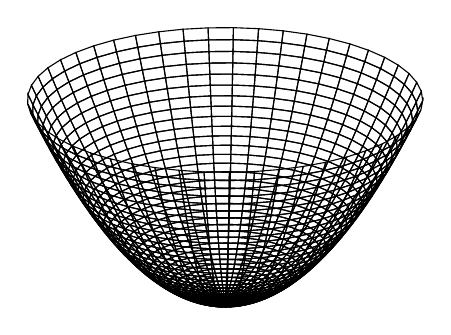
\begin{tikzpicture}
  \begin{axis}[
    view={30}{30},
    xlabel={$x$},
    ylabel={$y$},
    zlabel={$z$},
    axis lines=center,
    domain=0:2,
    y domain=0:360,
    samples=40,
    samples y=50,
    zmin=0, zmax=5,
    ymin=-2, ymax=2,
    enlargelimits=false,
    hide axis,
    colormap/cool,
    ]
    
    % Surface: rotate z = x^2 about z-axis
      \addplot3[
      mesh,
      draw=black,
      samples=40,
      samples y=50,
      domain=0:2,
      y domain=0:360,
      variable=\x,
      variable y=\t,
    ]
    ({\x*cos(\t)}, {\x*sin(\t)}, {\x^2});
    
  \end{axis}
\end{tikzpicture}
\captionof{figure}{Omdreiningsflate: $z = x^2+y^2$ $0\leq z\leq 4$}\label{fig:paraboloid}
\end{minipage}
\hfill
% Right: Cross-section in xz-plane
\begin{minipage}[t]{0.48\textwidth}
\centering
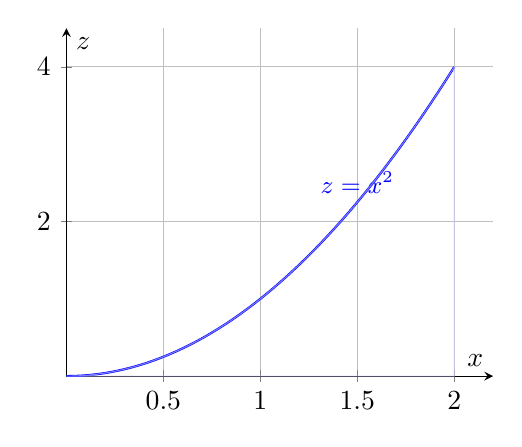
\begin{tikzpicture}
  \begin{axis}[
    xlabel={$x$},
    ylabel={$z$},
    axis lines=center,
    domain=0:2,
    samples=100,
    xmin=0, xmax=2.2,
    ymin=0, ymax=4.5,
    width=7cm,
    height=6cm,
    grid=major,
    enlargelimits=false,
    ]
    
    \addplot[thick, blue] {x^2};
    \node[blue] at (axis cs:1.5,2.5) {\small $z = x^2$};
    \addplot[blue!20, opacity=0.6, domain=0:2] {x^2} \closedcycle;
  \end{axis}
\end{tikzpicture}
\captionof{figure}{Snitt i $xz$-planet}\label{fig:snitt}
\end{minipage}
\end{figure}
Prosedyren for å parametrisere blir som følger:
\begin{enumerate}
\item sett $y=0$. Vi ser på snitt av flaten med $xz$-planet (se \Cref{fig:snitt}). Siden $z=x^2$ får vi $x=f(z):=\sqrt{z}$ for $0\leq z\leq 4$
\item Nå er parametrisering i sylinderkoordinater gitt som 
\[\vect{r}(\theta, z) = f(z)\cos (\theta) \vect{i}+f(z)\sin(\theta)\vect{j} + z\vect{k}, \quad 0\leq \theta\leq 2\pi,\ 0\leq z\leq 4\]
\end{enumerate}
Prosedyren beskrevet over fungerer også på andre omdreiningsflater. Vi valgte å legge polarkoordinatene i $xy$-planet, men dette var naturligvis et vilkårlig valg, basert på konvensjon. En kunne gjort et hvilket som helst annet valg, for deretter å velge rotasjonsakse normalt på det valgte polarkoordinat-planet. Men å begynne å rotere rundt en akse som ikke står normalt på polarkoordinatene vil ødelegge prosedyren over, og er frarådet. Da får man ikke utnyttet symmetrien i sylinderkoordinatene. Konklusjon: Roter rundt den aksen som står normalt på det valgte polarkoordinat-planet.

\subsection{Tangentplanet til en flate}
La oss se på hvordan vi finner tangentplanet til den parametriske flaten \( S \) gitt ved:
\[
\vect{r}(u, v) = x(u, v)\, \vect{i} + y(u, v)\, \vect{j} + z(u, v)\, \vect{k}
\]
Først definerer vi:
\begin{align*}
\vect{r}_u(u, v) = \frac{\partial x}{\partial u}(u, v)\, \vect{i} + \frac{\partial y}{\partial u}(u, v)\, \vect{j} + \frac{\partial z}{\partial u}(u, v)\, \vect{k}
\\
\vect{r}_v(u, v) = \frac{\partial x}{\partial v}(u, v)\, \vect{i} + \frac{\partial y}{\partial v}(u, v)\, \vect{j} + \frac{\partial z}{\partial v}(u, v)\, \vect{k}
\end{align*}
Vi kaller en parametrisering $\vect{r}$ \emph{regulær} hvis $\vect{r}_u, \vect{r}_v$ er lineært uavhengige for hvert punkt i domenet til $\vect{r}$.\footnote{Faktisk forutsetter alt som følger at vi jobber bare med regulære parametriseringer. De eksempler vi skal se på er alle valgt slik at det er oppfylt.}\smallskip

\begin{minipage}{7cm}
\textbf{Tangent i $v$-retning:}
Hvis vi holder\\ \( u = u_0 \) fast, vil \( \vect{r}_v(u_0, v) \) være tangent til kurven \( \vect{r}(u_0, v) \) (som faktisk er en kurve siden bare \( v \) varierer), forutsatt at \( \vect{r}_v(u_0, v) \neq \vect{0} \).\smallskip

\textbf{Tangent i $u$-retning}
Tilsvarende, hvis vi holder \( v = v_0 \) fast, vil \( \vect{r}_u(u, v_0) \) være tangent til kurven \( \vect{r}(u, v_0) \) (igjen en kurve siden bare \( u \) varierer), forutsatt at \( \vect{r}_u(u, v_0) \neq \vect{0} \).\smallskip

Både \( \vect{r}_u(u_0, v_0) \) og \( \vect{r}_v(u_0, v_0) \) vil (såfremt ingen av dem er nullvektoren) være tangenter til flaten \( S \) i punktet \( (u_0, v_0) \).

\textbf{Tangentplanet} til flaten i dette punktet er da planet som spenner over vektorene \( \vect{r}_u(u_0, v_0) \) og \( \vect{r}_v(u_0, v_0) \).
\end{minipage}
\begin{minipage}{7cm}
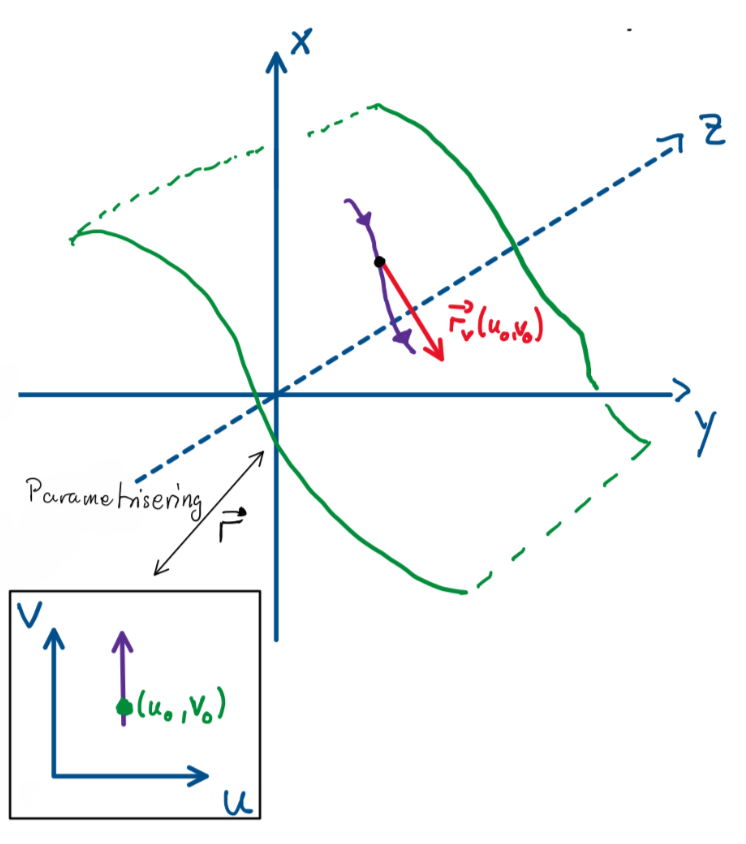
\includegraphics[width=7cm]{Fig/Tangent_vector.png}
\end{minipage}

Punktet $(u_0,v_0)$ i presentasjonen over er naturligvis vilkårlig. Resultatet gjelder for alle punkter der verken \( \vect{r}_u \) eller \( \vect{r}_v \) er nullvektorer.

Dette betyr at, så lenge \( \vect{r}_u \times \vect{r}_v \neq \vect{0} \), vil vektoren \( \vect{r}_u \times \vect{r}_v \) være ortogonal på flaten \( S \), og kan derfor brukes som normalvektor for å skrive ligningen til tangentplanet.

%\begin{minipage}{7.5cm}
\begin{defn}{Tangenter og normalvektorer}
Gitt en parametrisk flate \( \vect{r}(u,v) \), så kan vi finne \emph{tangentvektorer} til flaten ved å derivere med hensyn på hver parameter:
\[
\vect{r}_u = \frac{\partial \vect{r}}{\partial u}, \quad \vect{r}_v = \frac{\partial \vect{r}}{\partial v}
\]
Disse to vektorene ligger i tangentplanet til flaten (se \Cref{fig:tang_norm}), og kryssproduktet gir en vektor \emph{normal til flaten}:
\begin{align}
\label{nVec}
\vect{n} = \vect{r}_u \times \vect{r}_v
\end{align}
En slik vektor kaller vi \emph{normalenvektor}, og hvis vektoren har lengde $1$, sier vi at det er en \emph{enhetsnormalenvektor}.
\label{defn:tang_norm}
\end{defn}
%\end{minipage} \quad
\begin{figure}\centering
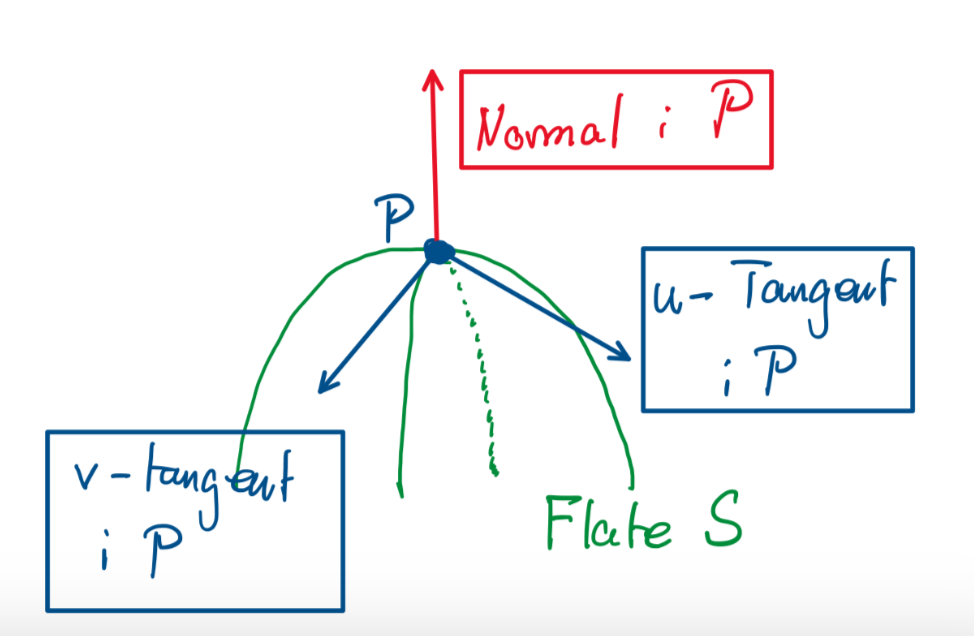
\includegraphics[width=10cm]{Fig/Tangents_Normal.png}\\
\caption{Tangentvektorer i et punkt $P$ på flaten $S$ sammen med normalenvektor. De to tangentvektorene spenner ut et tangentplan.}\label{fig:tang_norm}
\end{figure}

\begin{eks}{Flater som er grafer av funksjoner}
Hvis flaten er en grafen til en deriverbar funksjon $z=f(x,y)$ så kan vi alltid parametrisere flaten som

\begin{align}
\label{paramGraf}
\vect{r}(u,v)= u\vect{i}+v\vect{j}+f(u,v)\vect{k}
\end{align}
Vi har sett dette allerede for paraboloiden. Nå er det enkelt å beregne tangentvektor og normalvektor
\[\vect{r}_u =\vect{i}+f_u\vect{k} \quad \vect{r}_v=\vect{j}+f_v\vect{k} \quad \vect{n}=\vect{r}_u \times \vect{r}_v=\vect{k}-f_v\vect{j}-f_u\vect{i}\]
\label{ex:graf_flate}
\end{eks}

\subsection{Flateintegral på parameterflater}
Med dette verktøyet i bakhånd er vi nå beredt til å diskutere flateintegral. Med flateintegral mener vi her integralet av en funksjon over en flate. Tidligere, da vi så på dobbeltintegral, integrerte vi også over en flate, nemlig $xy$-planet (eller en av de andre koordinatplanene). Men et koordinatplan er en særdeles spesialisert flate. La oss minne oss selv på at det mentale bildet vi må basere intuisjonen på er et øyeblikksbilde av et laken i vinden\footnote{En av oss ville gjerne døpt om \textit{flateintegral} til \textit{lakenintegral}, for å presisere at man ikke nødvendigvis integrerer over et flatt domene. Vedkommende stiller seg uforstående til at dette ikke gikk igjennom. Vi beholder \textit{flateintegral}.}. I dette avsnittet skal vi altså integrere funksjoner over slike flater.
\begin{defn}{Flateintegral}
Anta at \( F \) er en flate som er parametrisert av $\vect{r}(u, v), (u,v)\in D$. Flateintegralet av en  funksjon $f(x,y,z)$ over en slik flate er da
\[\int_F f(\vect{r})\, dS := \iint_D f(\vect{r}(u,v))\lVert \vect{n}\rVert dA\]
hvor $D$ er parameterdomenet, slik at $(u,v)\in D$ og $\vect{n}$ er normalvektoren gitt i~\eqref{nVec}. Normen til normalvektoren er dermed gitt som 
\[\lVert \vect{n}\rVert=\lVert\vect{r}_u \times \vect{r}_v\rVert\]
\label{defn:flateintegral}
\end{defn}

\begin{oppsum}{Lagrange's triks for flateintegraler}
Flateintegraler bruker normen av normalenvektoren, som i tur er gitt som kryssproduktet av to tangenter. Det blir komplisert! Vi kan forenkle det hele ved å bruke Lagrange-formelen\footnote{I Lagrange-formelen skriver vi $\vect{x}^2 = \vect{x}\cdot \vect{x}$ hvor produktet er et prikkprodukt (skalarprodukt). Potenser av vektorer er sketchy greier (hvorfor?) men akkurat for potensen 2 så gir det en fiffig forkortelse som fungerer fint.}:
\[\lVert \vect{x} \times \vect{y}\rVert^2 = (\vect{x}\cdot \vect{x})(\vect{y}\cdot \vect{y})-(\vect{x}\cdot \vect{y})^2=\vect{x}^2\vect{y}^2-(\vect{x}\cdot \vect{y})^2\]
Dermed kan vi beregne uttrykk i flateintegralet enklere uten kryssprodukt som
\[\lVert \vect{r}_u \times \vect{r}_v\rVert=\sqrt{\vect{r}_u^2 \vect{r}_v^2 - (\vect{r}_u \cdot \vect{r}_v)^2}\]
\end{oppsum}
Vi kan nå benytte det vi har lært til å beregne arealet av parameterflater. 
\begin{defn}{Areal av parametriske flater}
Anta at \( F \) er en flate som er parametrisert av
$\vect{r}(u, v) , (u,v)\in D$. 
Forutsatt at \( S \) dekkes nøyaktig én gang når \( (u, v) \) går over alle punkter i området \( D \), er arealet til flaten \( S \) gitt ved:
\begin{align}\label{surfacearea}
\textrm{Areal} = \iint_S 1 dS = \iint_D\left\|\vect{n}\right\|dA=\iint_D \left\| \vect{r}_u \times \vect{r}_v \right\|\, dA = \iint_D \sqrt{\vect{r}_u^2  \vect{r}_v^2 - (\vect{r}_u \cdot \vect{r}_v)^2}\, dA
\end{align}
\end{defn}

\subsubsection{Tilbake til et spesialtilfelle: Arealet av overflaten til en graf}
La oss knytte en kommentar til spesialtilfellet hvor vi ser på overflaten til en graf. I det spesialtilfellet har vi altså at parametrene også er koordinatakser: $x=u,y=v$ og  $z=f(u,v)$. Dette svarer altså til å integrere grafen til $z=f(x,y)$ over $xy$-planet. Fra \Cref{ex:graf_flate}, så har vi at normalvektoren da er gitt som
\(\vect{n}=\vect{k}-f_y\vect{j}-f_x\vect{i},\) hvor vi minner om at f.eks. $f_y=\frac{\partial f}{\partial y}$.
Dette gir 
\[ \|\vect{n}\|=\sqrt{\vect{n}\cdot\vect{n}}=\sqrt{1+f_y^2+f_x^2}.\] Ved å sette dette inn i \Cref{surfacearea} så finner vi

\begin{align}\label{old_area_formel}
\textrm{Areal}= \iint_D \sqrt{ \left( \frac{\partial f}{\partial x} \right)^2 + \left( \frac{\partial f}{\partial y} \right)^2 + 1 }\, dA,
\end{align}
Om du nå blar tilbake kan du nå observere at dette er nøyaktig det samme som vi beregnet i \eqref{anv:flateareal}.

La oss i det følgende se på et eksempel.
\begin{eks}{Areal til del av en paraboloide med sirkulært tverrsnitt}\mbox{}\\
\begin{minipage}{7cm}
Flaten \( S \) er i dette tilfellet grafen til $f(x,y)=2-x^2-y^2$ og ligger over et område \( D = \{(x,y)^\top\in \R^2 \colon x^2+y^2 \leq 1\}\) i \( xy \)-planet. 
\end{minipage}
\begin{minipage}{5cm}
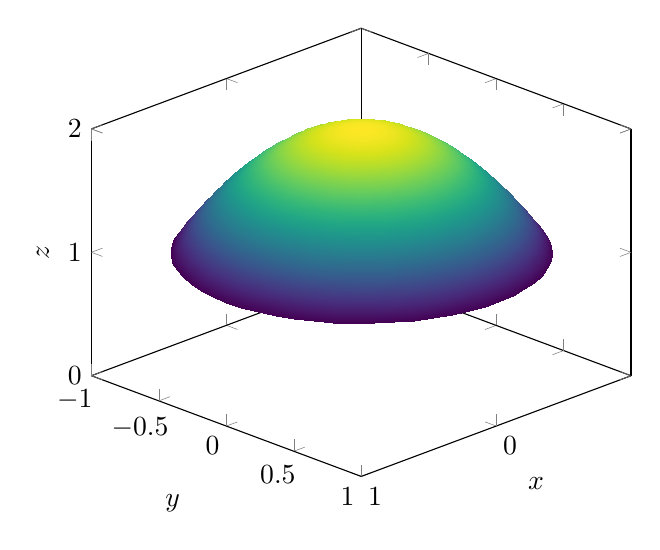
\begin{tikzpicture}
  \begin{axis}[
    view={135}{30},
    domain=0:1,
    domain y=0:360,
    samples=40,
    samples y=60,
    xlabel=$x$, ylabel=$y$, zlabel=$z$,
    colormap/viridis,
    z buffer=sort,
    zmin=0,
    zmax=2,
  ]
    % Convert from polar to Cartesian: x = r cos(θ), y = r sin(θ)
    \addplot3[
      surf,
      shader=interp,
      variable=\r,
    ]
    ({r*cos(y)}, {r*sin(y)}, {2 - r^2});
  \end{axis}
\end{tikzpicture}
\end{minipage}

Vi beregner de partiellderiverte til $f$ og får:
\[
\left\| \vect{r}_x \times \vect{r}_y \right\| = \sqrt{ \left( \frac{\partial f}{\partial x} \right)^2 + \left( \frac{\partial f}{\partial y} \right)^2 + 1 }=\sqrt{4x^2+4y^2+1}=\sqrt{4(x^2+y^2)+1}
\]
Rotasjonssymmetri gjør at vi velger sylinderkoordinater, hvor vi velger å legge polarkoordinat-planet i $xy$-planet. Da blir arealet
\begin{align*}
\iint_S dS &=\int_0^{2\pi}\int_{0}^1 \sqrt{4r^2+1}r\, drd\theta = \pi \int_0^1\sqrt{4u+1}\, du\\ &= \frac{\pi}{6} [(4u+1)^{3/2}]_0^1 =\frac{\pi}{6}(\sqrt{125}-1).
\end{align*}
\end{eks}
Merk at vi lot symmetri-betraktninger avgjøre hvilket koordinatsystem vi benyttet. Dersom integrasjonsområdet hadde hatt en annen form (et rektangel, for eksempel) eller dersom funksjonen ikke hadde hatt sylinder-symmetri, så ville vi kanskje gjort andre valg. 

I dette avsnittet har vi altså sett på flater gitt som grafen til en funksjon $z=f(x,y).$ Merk at vi selvsagt like gjerne kunne sett på flater definert over et av de andre koordinatplanene (altså integrasjonsdomene\( D \) i \( yz \)-planet eller \( xz \)-planet i stedet). 


\FloatBarrier